% Tell Rstudio this is a knitr document
% compile with: require(knitr); knit2pdf('fga2_303039534.Rnw')
\documentclass[12pt]{article}\usepackage[]{graphicx}\usepackage[]{color}
%% maxwidth is the original width if it is less than linewidth
%% otherwise use linewidth (to make sure the graphics do not exceed the margin)
\makeatletter
\def\maxwidth{ %
  \ifdim\Gin@nat@width>\linewidth
    \linewidth
  \else
    \Gin@nat@width
  \fi
}
\makeatother

\definecolor{fgcolor}{rgb}{0.345, 0.345, 0.345}
\newcommand{\hlnum}[1]{\textcolor[rgb]{0.686,0.059,0.569}{#1}}%
\newcommand{\hlstr}[1]{\textcolor[rgb]{0.192,0.494,0.8}{#1}}%
\newcommand{\hlcom}[1]{\textcolor[rgb]{0.678,0.584,0.686}{\textit{#1}}}%
\newcommand{\hlopt}[1]{\textcolor[rgb]{0,0,0}{#1}}%
\newcommand{\hlstd}[1]{\textcolor[rgb]{0.345,0.345,0.345}{#1}}%
\newcommand{\hlkwa}[1]{\textcolor[rgb]{0.161,0.373,0.58}{\textbf{#1}}}%
\newcommand{\hlkwb}[1]{\textcolor[rgb]{0.69,0.353,0.396}{#1}}%
\newcommand{\hlkwc}[1]{\textcolor[rgb]{0.333,0.667,0.333}{#1}}%
\newcommand{\hlkwd}[1]{\textcolor[rgb]{0.737,0.353,0.396}{\textbf{#1}}}%
\let\hlipl\hlkwb

\usepackage{framed}
\makeatletter
\newenvironment{kframe}{%
 \def\at@end@of@kframe{}%
 \ifinner\ifhmode%
  \def\at@end@of@kframe{\end{minipage}}%
  \begin{minipage}{\columnwidth}%
 \fi\fi%
 \def\FrameCommand##1{\hskip\@totalleftmargin \hskip-\fboxsep
 \colorbox{shadecolor}{##1}\hskip-\fboxsep
     % There is no \\@totalrightmargin, so:
     \hskip-\linewidth \hskip-\@totalleftmargin \hskip\columnwidth}%
 \MakeFramed {\advance\hsize-\width
   \@totalleftmargin\z@ \linewidth\hsize
   \@setminipage}}%
 {\par\unskip\endMakeFramed%
 \at@end@of@kframe}
\makeatother

\definecolor{shadecolor}{rgb}{.97, .97, .97}
\definecolor{messagecolor}{rgb}{0, 0, 0}
\definecolor{warningcolor}{rgb}{1, 0, 1}
\definecolor{errorcolor}{rgb}{1, 0, 0}
\newenvironment{knitrout}{}{} % an empty environment to be redefined in TeX

\usepackage{alltt}
\usepackage{mathpazo}
\usepackage{hyperref,url}
\usepackage[a4paper,margin=1.5cm]{geometry}
\usepackage{amsmath,amssymb,amsfonts,amsthm}

\newcommand{\Slang}{\texttt{S} }
\newcommand{\R}{\texttt{R} }
\newcommand{\Rfunction}[1]{{\texttt{#1}}}
\newcommand{\Robject}[1]{{\texttt{#1}}}
\newcommand{\Rpackage}[1]{{\mbox{\normalfont\textsf{#1}}}}

\usepackage{xcolor}
\definecolor{Red}{rgb}{0.7,0,0}
\definecolor{Blue}{rgb}{0,0,0.8}

\usepackage{hyperref}
\hypersetup{%
  pdfusetitle,
  bookmarks = {true},
  bookmarksnumbered = {true},
  bookmarksopen = {true},
  bookmarksopenlevel = 2,
  unicode = {true},
  breaklinks = {false},
  hyperindex = {true},
  colorlinks = {true},
  linktocpage = {true},
  plainpages = {false},
  linkcolor = {Blue},
  citecolor = {Blue},
  urlcolor = {Red},
  pdfstartview = {Fit},
  pdfpagemode = {UseOutlines},
  pdfview = {XYZ null null null}
}

\setlength{\parindent}{0in}

\usepackage{titling}
\usepackage{titlesec}
\titleformat*{\section}{\large\bfseries}
\titlespacing\section{0pt}{10pt plus 4pt minus 2pt}{0pt plus 2pt minus 2pt}
\titlespacing\subsection{0pt}{12pt plus 4pt minus 2pt}{0pt plus 2pt minus 2pt}
\titlespacing\subsubsection{0pt}{12pt plus 4pt minus 2pt}{0pt plus 2pt minus 2pt}
\IfFileExists{upquote.sty}{\usepackage{upquote}}{}
\begin{document}

\begin{center}
\textbf{\Large{\centering{FG Assignment 2}}}\\
\textit{USN: 303039534}
\end{center}



\section*{2\quad Simulating Copy Number Profiles}

We start by writing a function cnv\_sim(N) that simulates N copy number changes from an initially homogenous human genome using the function cn\_change to generate each copy number change. We initiate each change uniformly at random along the genome. Since a higher copy number implies more of a particular DNA sequence, we need to weigh our sampling by the copy number. This also ensures that once a sequence has a copy number of zero, the loss of information is irreversible since in this case we are multiplying our probabilities by zero. The probabilty of a copy number change occuring in segment i is thus given by\\
\begin{equation*}
p_i = \frac{L_i \cdot cn_i}{\sum_j{L_j \cdot cn_j}}
\end{equation*}
Here, $L_i$ and $cn_i$ is the length and copy number of segment i respectively. After picking a segment, we pick the initiation site uniformly at random within the segment. The length of a copy number change is drawn uniformly at random from a distribution ranging from 1 to 100 Mb. We let the change extend symmetrically around the initation site but bounded by the beginning and end of the segment in which it occurs. This implementation is roughly equivalent to assuming that a break is equally likely between any two bases in any chromosome, but with a bias towards changes extending to the end of a segment and towards smaller segments due to the hard segment cut-off. Real biological systems are more complex than this, but it is sufficient for the purpose of verifying our algorithm in sections 7 and 8. The simulation is run on a dataframe storing the chromosome, length and copy number of each segment. Segments are stored in order along the genome which allows us to reconstruct the full genome from our segments. For all of our simulations, we assume the samples to be female to avoid complications in assigning initial X and Y copy numbers for multiploid genomes. However, the code can easily be extended to also initialize Y chromosomes.


\begin{kframe}
\begin{alltt}
\hlkwd{set.seed}\hlstd{(}\hlnum{26110940}\hlstd{)} \hlcom{#set seed for repeatable simulations}
\hlstd{chr_size_file} \hlkwb{=} \hlstr{'hg19.chrom.sizes.txt'} \hlcom{#change if different file name}

\hlstd{cn_change} \hlkwb{=} \hlkwa{function}\hlstd{(}\hlkwc{results}\hlstd{,} \hlkwc{tot.size}\hlstd{,} \hlkwc{n_change}\hlstd{)\{}
  \hlcom{#simulates a single copy number change given a data frame of segments (results)}
  \hlcom{#a cn change is initiated uniformly at random across the genome}
  \hlcom{#it then extends symmetrically in both directions with a length}
  \hlcom{#of 1-100 Mb picked uniformly at random, bounded by the segment boundaries}
  \hlcom{#tot.size is the total genome size in basepairs, n_change the max cn change}

  \hlcom{#probability of initating a cn change at each basepair}
  \hlcom{#is proportional to its length and current copy number}
  \hlstd{ps} \hlkwb{=} \hlkwd{cumsum}\hlstd{(} \hlkwd{c}\hlstd{(}\hlnum{0}\hlstd{, results[,}\hlstr{'length'}\hlstd{]}\hlopt{*}\hlstd{results[,}\hlstr{'cn'}\hlstd{])} \hlopt{/} \hlstd{tot.size )}
  \hlstd{pos} \hlkwb{=} \hlkwd{runif}\hlstd{(}\hlnum{1}\hlstd{)}
  \hlcom{#first find segment in which a CN change occurs, then the point of change}
  \hlstd{seg} \hlkwb{=} \hlkwd{sum} \hlstd{(}\hlkwd{as.numeric}\hlstd{(pos} \hlopt{>} \hlstd{ps)); chr} \hlkwb{=} \hlkwd{as.character}\hlstd{(results[seg,} \hlstr{'chr'}\hlstd{]);}
  \hlstd{L} \hlkwb{=} \hlstd{results[seg,} \hlstr{'length'}\hlstd{]}

  \hlstd{site} \hlkwb{=} \hlkwd{round}\hlstd{(}\hlkwd{runif}\hlstd{(}\hlnum{1}\hlstd{)}\hlopt{*}\hlstd{L,}\hlnum{0}\hlstd{); size} \hlkwb{=} \hlkwd{round}\hlstd{(}\hlkwd{runif}\hlstd{(}\hlnum{1}\hlstd{,} \hlnum{10}\hlopt{^}\hlnum{6}\hlstd{,} \hlnum{10}\hlopt{^}\hlnum{8}\hlstd{),} \hlnum{0}\hlstd{)}
  \hlstd{init} \hlkwb{=} \hlkwd{max}\hlstd{(}\hlnum{1}\hlstd{, site}\hlopt{-}\hlkwd{floor}\hlstd{(size}\hlopt{/}\hlnum{2}\hlstd{))} \hlcom{#cn change cannot go past segment start}
  \hlstd{fin} \hlkwb{=} \hlkwd{min}\hlstd{(L, site}\hlopt{+}\hlkwd{ceiling}\hlstd{(size}\hlopt{/}\hlnum{2}\hlstd{))} \hlcom{#cn change cannot go past segment end}

  \hlstd{change} \hlkwb{=} \hlkwd{sample}\hlstd{(} \hlkwd{c}\hlstd{(} \hlopt{-}\hlstd{n_change}\hlopt{:-}\hlnum{1} \hlstd{,} \hlnum{1}\hlopt{:}\hlstd{n_change ),} \hlnum{1}\hlstd{)}
  \hlstd{new_cn} \hlkwb{=} \hlstd{results[seg,}\hlstr{'cn'}\hlstd{]}\hlopt{+}\hlstd{change} \hlcom{#old copy number plus change}
  \hlstd{new_cn} \hlkwb{=} \hlkwd{max}\hlstd{(}\hlnum{0}\hlstd{, new_cn)} \hlcom{# don't allow negative copy numbers}
  \hlstd{tot.size} \hlkwb{=} \hlstd{tot.size} \hlopt{+} \hlstd{change}\hlopt{*}\hlstd{(fin}\hlopt{-}\hlstd{init)} \hlcom{#update our total amount of DNA}

  \hlkwa{if} \hlstd{(} \hlkwd{isTRUE}\hlstd{(}\hlkwd{all.equal}\hlstd{(} \hlkwd{c}\hlstd{(init,fin),} \hlkwd{c}\hlstd{(}\hlnum{1}\hlstd{,L) ) ))\{} \hlcom{#complete overlap, update cn}
    \hlstd{results[seg,}\hlstr{'cn'}\hlstd{]}\hlkwb{=}\hlstd{new_cn}
  \hlstd{\}}\hlkwa{else if} \hlstd{(init} \hlopt{==} \hlnum{1}\hlstd{)\{} \hlcom{#creates new CN at start of segment}
    \hlstd{results[seg,}\hlstr{'length'}\hlstd{]} \hlkwb{=} \hlstd{L} \hlopt{-} \hlstd{fin}
    \hlkwa{if}\hlstd{(seg}\hlopt{==}\hlnum{1}\hlstd{)\{results} \hlkwb{=} \hlkwd{rbind}\hlstd{(}\hlkwd{list}\hlstd{(chr, fin, new_cn), results)}
    \hlstd{\}}\hlkwa{else}\hlstd{\{results} \hlkwb{=} \hlkwd{rbind}\hlstd{(results[}\hlnum{1}\hlopt{:}\hlstd{(seg}\hlopt{-}\hlnum{1}\hlstd{),],}
                          \hlkwd{list}\hlstd{(chr, fin, new_cn), results[}\hlopt{-}\hlstd{(}\hlnum{1}\hlopt{:}\hlstd{(seg}\hlopt{-}\hlnum{1}\hlstd{)),])\}}
  \hlstd{\}}\hlkwa{else if} \hlstd{(fin} \hlopt{==} \hlstd{L)\{} \hlcom{#new CN at end of segment}
    \hlstd{results[seg,}\hlstr{'length'}\hlstd{]} \hlkwb{=} \hlstd{init}
    \hlstd{results} \hlkwb{=} \hlkwd{rbind}\hlstd{(results[}\hlnum{1}\hlopt{:}\hlstd{seg,],} \hlkwd{list}\hlstd{(chr, L}\hlopt{-}\hlstd{init, new_cn), results[}\hlopt{-}\hlstd{(}\hlnum{1}\hlopt{:}\hlstd{seg),])}
  \hlstd{\}}\hlkwa{else}\hlstd{\{} \hlcom{#cn change falls within segment}
    \hlkwa{if}\hlstd{(seg} \hlopt{==} \hlnum{1}\hlstd{)\{results} \hlkwb{=} \hlkwd{rbind}\hlstd{(results[}\hlnum{1}\hlstd{,],} \hlkwd{list}\hlstd{(chr, size, new_cn), results)}
    \hlstd{\}}\hlkwa{else}\hlstd{\{results} \hlkwb{=} \hlkwd{rbind}\hlstd{(results[}\hlnum{1}\hlopt{:}\hlstd{seg,],}
                          \hlkwd{list}\hlstd{(chr, size, new_cn), results[}\hlopt{-}\hlstd{(}\hlnum{1}\hlopt{:}\hlstd{(seg}\hlopt{-}\hlnum{1}\hlstd{)),])\}}
    \hlstd{results[seg,}\hlstr{'length'}\hlstd{]}\hlkwb{=} \hlstd{init}
    \hlstd{results[seg}\hlopt{+}\hlnum{2}\hlstd{,}\hlstr{'length'}\hlstd{]}\hlkwb{=} \hlstd{L}\hlopt{-}\hlstd{fin}
  \hlstd{\}}
  \hlkwd{return}\hlstd{(}\hlkwd{list}\hlstd{(results, tot.size))}
\hlstd{\}}

\hlstd{cnv_sim} \hlkwb{=} \hlkwa{function}\hlstd{(}\hlkwc{N}\hlstd{,} \hlkwc{n_change} \hlstd{=} \hlnum{1}\hlstd{,} \hlkwc{noise} \hlstd{=} \hlnum{0}\hlstd{,} \hlkwc{ploidy}\hlstd{=}\hlnum{2}\hlstd{)\{}
  \hlcom{#simulates N copy number changes in a hypothetical human genome}
  \hlcom{#n_change is max copy number change in a single event}
  \hlcom{#noise specifies whether we add Gaussian noise, ploidy specifies initial ploidy}
  \hlcom{#we assume samples to be female}
  \hlstd{results} \hlkwb{=} \hlkwd{read.table}\hlstd{(chr_size_file,} \hlkwc{stringsAsFactors} \hlstd{=} \hlnum{0}\hlstd{)}
  \hlstd{results[,}\hlnum{3}\hlstd{]} \hlkwb{=} \hlkwd{rep}\hlstd{(ploidy,}\hlnum{24}\hlstd{)} \hlcom{#initialize genome}
  \hlkwd{colnames}\hlstd{(results)} \hlkwb{=} \hlkwd{c}\hlstd{(}\hlstr{'chr'}\hlstd{,} \hlstr{'length'}\hlstd{,} \hlstr{'cn'}\hlstd{)}
  \hlstd{results[results[,}\hlstr{'chr'}\hlstd{]} \hlopt{==} \hlstr{'chrY'}\hlstd{,} \hlstr{'cn'}\hlstd{]} \hlkwb{=} \hlnum{0} \hlcom{#assume female}
  \hlstd{tot.size} \hlkwb{=} \hlstd{ploidy}\hlopt{*}\hlnum{3036303846} \hlcom{#total number of base pairs}
  \hlkwa{for} \hlstd{(i} \hlkwa{in} \hlnum{1}\hlopt{:}\hlstd{N)\{}
    \hlstd{new_res} \hlkwb{=} \hlkwd{cn_change}\hlstd{(results, tot.size, n_change)} \hlcom{#simulate cn change}
    \hlstd{results} \hlkwb{=} \hlstd{new_res[[}\hlnum{1}\hlstd{]]; tot.size} \hlkwb{=} \hlstd{new_res[[}\hlnum{2}\hlstd{]]}
  \hlstd{\}}
  \hlkwd{colnames}\hlstd{(results)}\hlkwb{=}\hlkwd{c}\hlstd{(}\hlstr{'chr'}\hlstd{,} \hlstr{'length'}\hlstd{,} \hlstr{'cn'}\hlstd{);} \hlkwd{rownames}\hlstd{(results)}\hlkwb{=}\hlnum{1}\hlopt{:}\hlkwd{dim}\hlstd{(results)[}\hlnum{1}\hlstd{]}
  \hlcom{#Add Gaussian noise to all segments if specified}
  \hlkwa{if} \hlstd{(noise)\{ results[,}\hlnum{3}\hlstd{]} \hlkwb{=} \hlstd{results[,}\hlnum{3}\hlstd{]} \hlopt{+} \hlkwd{rnorm}\hlstd{(}\hlkwd{dim}\hlstd{(results)[}\hlnum{1}\hlstd{],} \hlkwc{sd}\hlstd{=}\hlnum{0.1}\hlstd{) \}}
  \hlkwd{return}\hlstd{(results)}
\hlstd{\}}
\end{alltt}
\end{kframe}

The first 10 segments of an example simulation of 50 copy number changes are given in table \ref{tab:sim}.\\

\begin{kframe}
\begin{alltt}
\hlstd{res} \hlkwb{=} \hlkwd{cnv_sim}\hlstd{(}\hlnum{50}\hlstd{,} \hlkwc{n_change} \hlstd{=} \hlnum{1}\hlstd{,} \hlkwc{noise} \hlstd{=} \hlnum{0}\hlstd{,} \hlkwc{ploidy}\hlstd{=}\hlnum{2}\hlstd{)}
\hlstd{xres} \hlkwb{=} \hlkwd{xtable}\hlstd{(res[}\hlnum{1}\hlopt{:}\hlnum{10}\hlstd{,],}
              \hlkwc{caption} \hlstd{=} \hlstr{'First 10 segments following 
              a simulation of 50 copy number changes'}\hlstd{,}
              \hlkwc{digits}\hlstd{=}\hlkwd{c}\hlstd{(}\hlnum{0}\hlstd{,}\hlnum{0}\hlstd{,}\hlnum{0}\hlstd{,}\hlnum{0}\hlstd{),} \hlkwc{label}\hlstd{=}\hlstr{'tab:sim'}\hlstd{)}
\hlstd{addtorow} \hlkwb{=} \hlkwd{list}\hlstd{()}
\hlstd{addtorow}\hlopt{$}\hlstd{pos} \hlkwb{=} \hlkwd{list}\hlstd{(}\hlnum{0}\hlstd{)}
\hlstd{addtorow}\hlopt{$}\hlstd{command} \hlkwb{<-} \hlkwd{c}\hlstd{(}\hlstr{' Segment & Chromosome & Length & Copy Number \textbackslash{}\textbackslash{}\textbackslash{}\textbackslash{}\textbackslash{}n'} \hlstd{)}
\hlkwd{align}\hlstd{(xres)} \hlkwb{<-} \hlkwd{rep}\hlstd{(}\hlstr{"r"}\hlstd{,} \hlnum{4}\hlstd{)}
\hlkwd{print}\hlstd{(xres,} \hlkwc{include.colnames} \hlstd{=} \hlnum{0}\hlstd{,} \hlkwc{add.to.row} \hlstd{= addtorow)}
\end{alltt}
\end{kframe}% latex table generated in R 3.5.0 by xtable 1.8-3 package
% Sun Dec  2 16:23:08 2018
\begin{table}[ht]
\centering
\begin{tabular}{rrrr}
  \hline
   Segment & Chromosome & Length & Copy Number \\
 \hline
1 & chr1 & 70934013 & 2 \\ 
  2 & chr1 & 22654494 & 3 \\ 
  3 & chr1 & 93777278 & 2 \\ 
  4 & chr1 & 27836603 & 1 \\ 
  5 & chr1 & 9107794 & 2 \\ 
  6 & chr1 & 24940439 & 2 \\ 
  7 & chr2 & 20398012 & 2 \\ 
  8 & chr2 & 11119108 & 3 \\ 
  9 & chr2 & 10134647 & 3 \\ 
  10 & chr2 & 116703974 & 2 \\ 
   \hline
\end{tabular}
\caption{First 10 segments following 
              a simulation of 50 copy number changes} 
\label{tab:sim}
\end{table}


We also write a function plot\_results() to visualize the resulting genomic profile and a function sim\_more\_cnvs() to simulate multiple copy number changes and plot the resulting profiles. 

\begin{knitrout}
\definecolor{shadecolor}{rgb}{0.969, 0.969, 0.969}\color{fgcolor}\begin{kframe}
\begin{alltt}
\hlstd{plot_results} \hlkwb{=} \hlkwa{function}\hlstd{(}\hlkwc{results}\hlstd{,} \hlkwc{ploidy}\hlstd{=}\hlstr{'NA'}\hlstd{,} \hlkwc{n_change}\hlstd{=}\hlstr{'NA'}\hlstd{,} \hlkwc{noise}\hlstd{=}\hlnum{2}\hlstd{,} \hlkwc{main}\hlstd{=}\hlstr{''}\hlstd{)\{}
  \hlcom{#given a dataframe of segment lengths and cns, plots copy number profile}
  \hlstd{cum} \hlkwb{=} \hlkwd{cumsum}\hlstd{(results[,}\hlnum{2}\hlstd{])} \hlcom{#x boundaries}
  \hlstd{ymax} \hlkwb{=} \hlkwd{min}\hlstd{(} \hlkwd{max}\hlstd{(results[,}\hlnum{3}\hlstd{],} \hlkwc{na.rm}\hlstd{=T)}\hlopt{+}\hlnum{1}\hlstd{,} \hlkwd{median}\hlstd{(results[,}\hlnum{3}\hlstd{],} \hlkwc{na.rm}\hlstd{=}\hlnum{1}\hlstd{)}\hlopt{+}\hlnum{5}\hlstd{)}
  \hlkwd{plot}\hlstd{(}\hlkwd{c}\hlstd{(}\hlnum{1}\hlstd{,} \hlnum{3095677412}\hlstd{),} \hlkwd{c}\hlstd{(}\hlnum{2}\hlstd{,}\hlnum{2}\hlstd{),} \hlkwc{type}\hlstd{=}\hlstr{'n'}\hlstd{,} \hlkwc{lty}\hlstd{=}\hlnum{2}\hlstd{,}
       \hlkwc{xlim} \hlstd{=} \hlkwd{c}\hlstd{(}\hlnum{1}\hlstd{,} \hlnum{3095677412}\hlstd{),} \hlkwc{ylim} \hlstd{=} \hlkwd{c}\hlstd{(}\hlopt{-}\hlnum{0.5}\hlstd{, ymax),}
       \hlkwc{xlab} \hlstd{=} \hlstr{''}\hlstd{,} \hlkwc{ylab} \hlstd{=} \hlstr{''}\hlstd{,} \hlkwc{main} \hlstd{= main,} \hlkwc{xaxt} \hlstd{=} \hlstr{'n'}
       \hlstd{)} \hlcom{#initialize plot}

  \hlkwd{segments}\hlstd{(} \hlnum{1}\hlstd{,} \hlkwd{seq}\hlstd{(}\hlnum{0}\hlstd{,} \hlkwd{floor}\hlstd{(ymax),} \hlnum{1}\hlstd{),} \hlcom{#plot integer lines}
            \hlkwc{x1} \hlstd{=} \hlnum{3095677412}\hlstd{,} \hlkwc{y1} \hlstd{=} \hlkwd{seq}\hlstd{(}\hlnum{0}\hlstd{,} \hlkwd{floor}\hlstd{(ymax),} \hlnum{1}\hlstd{),} \hlkwc{lwd}\hlstd{=}\hlnum{0.2}\hlstd{,} \hlkwc{lty}\hlstd{=}\hlnum{2}  \hlstd{)}
  \hlkwd{segments}\hlstd{(} \hlkwd{c}\hlstd{(}\hlnum{0}\hlstd{, cum[}\hlopt{-}\hlkwd{length}\hlstd{(cum)]), results[,} \hlnum{3}\hlstd{],} \hlcom{#plot copy numbers}
            \hlkwc{x1} \hlstd{= cum,} \hlkwc{col}\hlstd{=}\hlstr{'blue'}\hlstd{,} \hlkwc{y1} \hlstd{= results[,} \hlnum{3}\hlstd{],} \hlkwc{lwd}\hlstd{=}\hlnum{3}  \hlstd{)}

  \hlstd{chr_sizes} \hlkwb{=} \hlkwd{read.table}\hlstd{(chr_size_file)}
  \hlstd{cum} \hlkwb{=} \hlkwd{cumsum}\hlstd{(}\hlkwd{as.numeric}\hlstd{(chr_sizes[,}\hlnum{2}\hlstd{])); cum} \hlkwb{=} \hlstd{cum[}\hlopt{-}\hlkwd{length}\hlstd{(cum)]}
  \hlkwd{segments}\hlstd{( cum,} \hlopt{-}\hlnum{0.5}\hlstd{,} \hlkwc{x1} \hlstd{= cum, ymax,} \hlkwc{lwd}\hlstd{=}\hlnum{0.5}\hlstd{)} \hlcom{#plot chromosome delineations}
\hlstd{\}}

\hlstd{sim_more_cnvs} \hlkwb{=} \hlkwa{function}\hlstd{(}\hlkwc{cnvs} \hlstd{=} \hlkwd{c}\hlstd{(}\hlnum{3}\hlstd{,}\hlnum{10}\hlstd{,}\hlnum{25}\hlstd{,}\hlnum{100}\hlstd{,}\hlnum{200}\hlstd{),} \hlkwc{n_change}\hlstd{=}\hlnum{1}\hlstd{,} \hlkwc{noise}\hlstd{=}\hlnum{0}\hlstd{,} \hlkwc{ploidy}\hlstd{=}\hlnum{2}\hlstd{)\{}
  \hlcom{#function for simulating multiple CNVs and putting in a plot}
  \hlkwd{par}\hlstd{(}\hlkwc{mfrow}\hlstd{=}\hlkwd{c}\hlstd{(}\hlkwd{length}\hlstd{(cnvs),}\hlnum{1}\hlstd{),} \hlkwc{mar}\hlstd{=}\hlkwd{c}\hlstd{(}\hlnum{0.5}\hlstd{,}\hlnum{2.5}\hlstd{,}\hlnum{0.5}\hlstd{,}\hlnum{1}\hlstd{),} \hlkwc{xaxs}\hlstd{=}\hlstr{'i'}\hlstd{,} \hlkwc{yaxs}\hlstd{=}\hlstr{'i'}\hlstd{,} \hlkwc{lend}\hlstd{=}\hlnum{1}\hlstd{)}
  \hlstd{results} \hlkwb{=} \hlkwd{vector}\hlstd{(}\hlstr{'list'}\hlstd{,} \hlnum{0}\hlstd{)}
  \hlkwa{for} \hlstd{(cnv} \hlkwa{in} \hlstd{cnvs)\{}
    \hlstd{results[[cnv]]} \hlkwb{=} \hlkwd{cnv_sim}\hlstd{(cnv, n_change, noise, ploidy)} \hlcom{#simulate changes}
    \hlkwd{plot_results}\hlstd{(results[[cnv]], ploidy, n_change, noise)} \hlcom{#plot result}
  \hlstd{\}}
  \hlkwd{return}\hlstd{(results)}
\hlstd{\}}
\end{alltt}
\end{kframe}
\end{knitrout}

\newpage
Using these functions, we simulate and plot genomic profiles with 3, 10, 25, 100 and 200 copy number changes (figure \ref{fig:no_noise}) from a diploid genome. In this and all subsequent plots, the x-axis indicates genomic posision with chromosomes ordered from 1:22 followed by the X and Y chromsomes. The beginning and end of each chromosome is indicated by a vertical line.

\begin{figure}[h!]
  \centering
\begin{knitrout}
\definecolor{shadecolor}{rgb}{0.969, 0.969, 0.969}\color{fgcolor}\begin{kframe}
\begin{alltt}
\hlstd{res1} \hlkwb{=} \hlkwd{sim_more_cnvs}\hlstd{(} \hlkwc{noise}\hlstd{=}\hlnum{FALSE}\hlstd{,} \hlkwc{n_change}\hlstd{=}\hlnum{1}\hlstd{)}
\end{alltt}
\end{kframe}
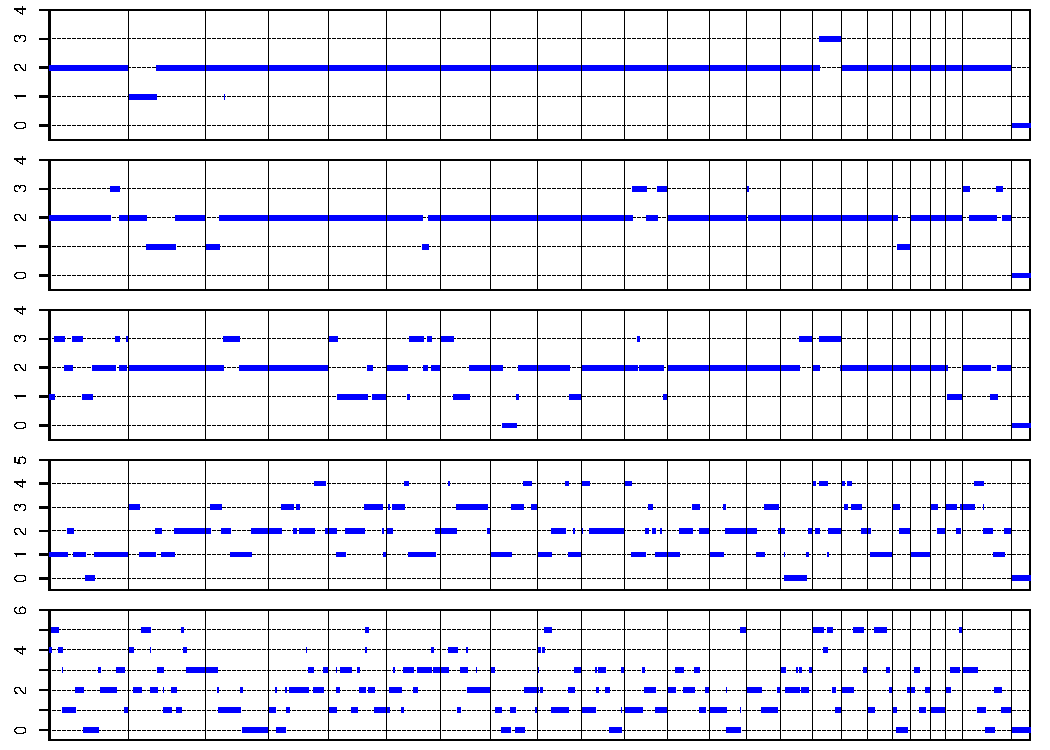
\includegraphics[width=.95\linewidth]{figure/unnamed-chunk-5-1} 

\end{knitrout}
\caption{Simulated copy number profiles after 3 (top), 10, 25, 100 and 200 (bottom) copy number changes. The y axis indicates absolute copy number, the x axis indicates position in the human genome. Vertical lines indicate chromosome boundaries with chromosomes ordered from 1:22 followed by the X and Y chromosomes.}
\label{fig:no_noise}
\end{figure}

\newpage
\section*{3\quad Introducing Noise}

We can simulate segmentation noise with our sim\_cnv() function by introducing Gaussian noise with a standard deviation of 0.1 to all segments. We can also allow for copy number changes of more than one copy per change. This is specified by providing the optional argument n\_change to sim\_cnv(). In this case, copy number changes are drawn randomly from positive or negative integer values ranging from 1 to n\_change without allowing changes that would lead to negative copy numbers. Copy number profiles for simulations of 3, 10, 25, 100 and 200 copy number changes with Gaussian noise and n\_change = 2 are given in figure \ref{fig:noise}.

\begin{figure}[h!]
  \centering
\begin{knitrout}
\definecolor{shadecolor}{rgb}{0.969, 0.969, 0.969}\color{fgcolor}\begin{kframe}
\begin{alltt}
\hlstd{res2} \hlkwb{=} \hlkwd{sim_more_cnvs}\hlstd{(} \hlkwc{noise}\hlstd{=}\hlnum{TRUE}\hlstd{,} \hlkwc{n_change}\hlstd{=}\hlnum{2}\hlstd{)}
\end{alltt}
\end{kframe}
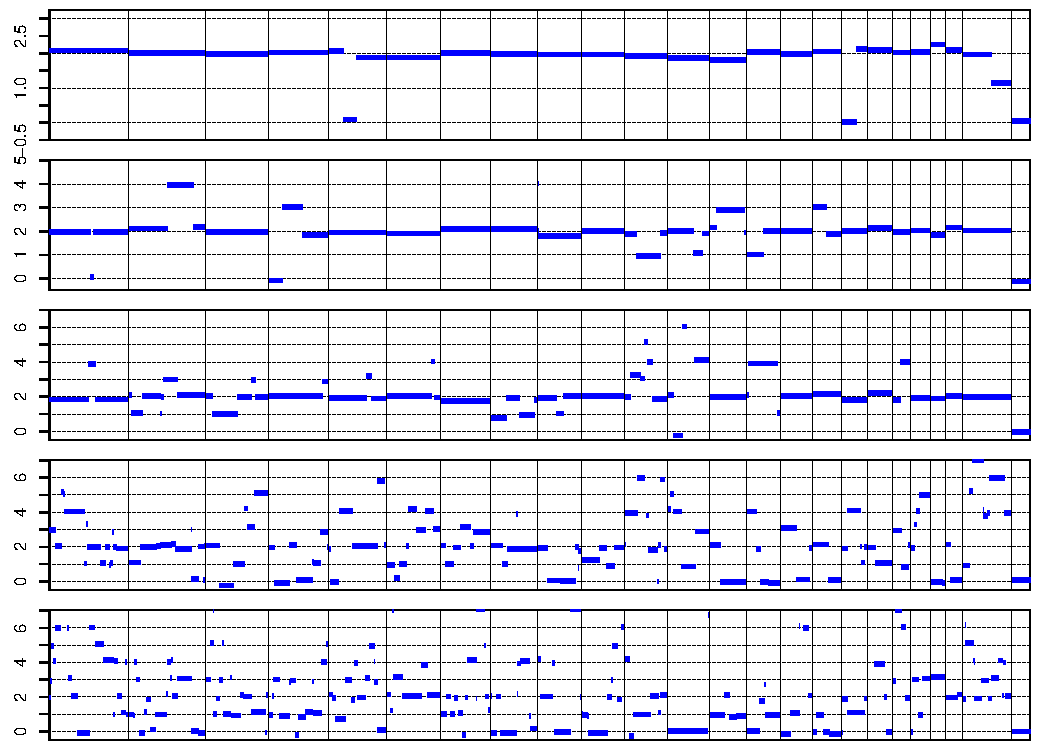
\includegraphics[width=.95\linewidth]{figure/unnamed-chunk-6-1} 

\end{knitrout}
\caption{Copy number profiles for simulations including segmentation noise and n\_change = 2. The number of copy number changes for the profiles are 3 (top), 10, 25, 100 and 200 (bottom).}
\label{fig:noise}
\end{figure}

\newpage

\section*{4\quad Altering Background Ploidy}

Many tumor cells have undergone full genome duplications, and we may thus want to simulate copy number changes from a reference genome that is not diploid. We achieve this by introducing the optional argument 'ploidy' with a default value of 2, specifying the ploidy of our reference genome. Setting ploidy=4, we simulate copy number changes from a tetraploid genome with the resulting genomic profiles given in figure \ref{fig:tetraploid}.

\begin{figure}[h!]
  \centering
\begin{knitrout}
\definecolor{shadecolor}{rgb}{0.969, 0.969, 0.969}\color{fgcolor}\begin{kframe}
\begin{alltt}
\hlstd{res3} \hlkwb{=} \hlkwd{sim_more_cnvs}\hlstd{(} \hlkwc{noise}\hlstd{=}\hlnum{TRUE}\hlstd{,} \hlkwc{n_change}\hlstd{=}\hlnum{2}\hlstd{,} \hlkwc{ploidy}\hlstd{=}\hlnum{4}\hlstd{)}
\end{alltt}
\end{kframe}
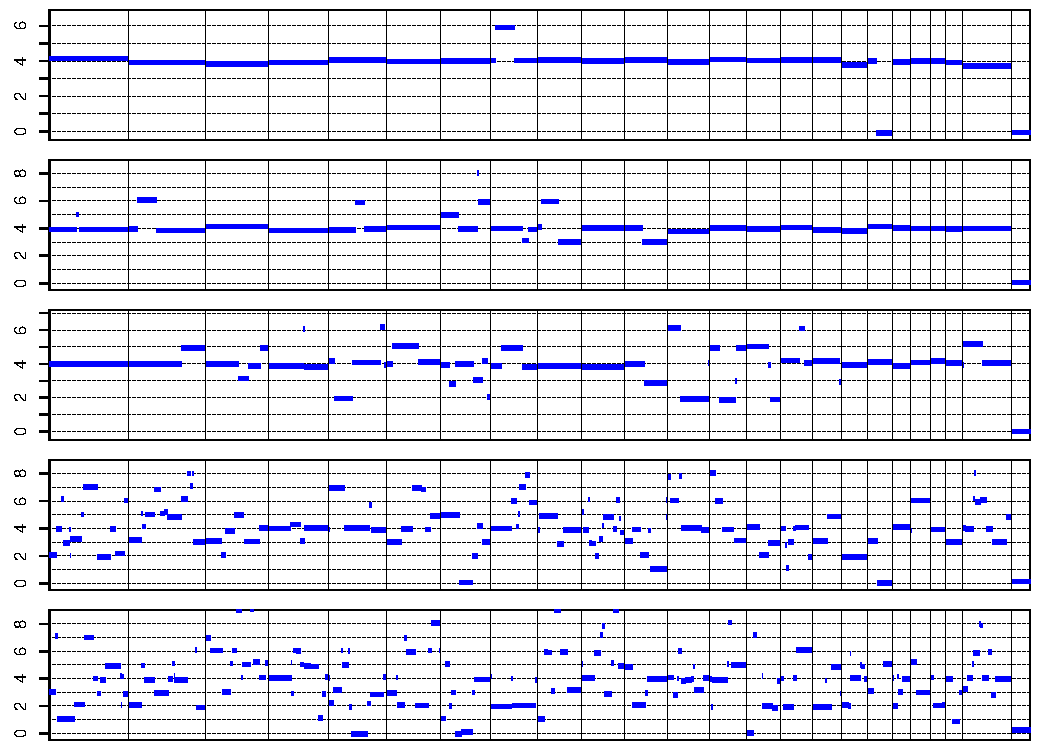
\includegraphics[width=.95\linewidth]{figure/unnamed-chunk-7-1} 

\end{knitrout}
\caption{Copy number profiles for copy number changes from a tetraploid chromosome, including segmentation noise and with n\_change = 2. The number of copy number changes for the profiles are 3 (top), 10, 25, 100 and 200 (bottom).}
\label{fig:tetraploid}
\end{figure}

\newpage

\section*{5\quad Normalization and Assessing Clonal Similarity}

We proceed to write a function normalize() to normalize these absolute copy number values by the median copy number value to simulate the relative copy number data we get from experiments. We also write a function clonal\_proximity() that assesses how close a given copy number profile is to being clonal (i.e. to having integer copy numbers). This is quantified using a Euclidean clonal distance metric weighted by segment length:
\begin{equation*}
d = \sqrt{ ( \sum_i{cn_i - \text{round}(cn_i, 0) )^2 \cdot L_i } ) \cdot \frac{4}{L} }
\end{equation*}
I.e. we consider how far the copy number of each segment is from being an integer, weigh this by the segment length, and normalize by the total genome size L. Weighting by segment length ensures that each position in the genome contributes equally to the distance metric, and using a Euclidean distance was found to yield better results than a linear (Manhattan) or higher power distance. This clonal distance is 0 if all segments have an integer copy number and 1 if all segments have half-integer copy numbers. We therefore define a normalized clonal similarity metric as $sim = 1-d$ which also runs from 0 to 1.
Finally, we write a function test\_proximity() that takes as input a dataframe of relative copy number data for a set of segments, scales the copy numbers linearly, and finds the scaling factor that optimizes the clonal similarity metric. This gives an estimate of absolute copy numbers.

\begin{knitrout}
\definecolor{shadecolor}{rgb}{0.969, 0.969, 0.969}\color{fgcolor}\begin{kframe}
\begin{alltt}
\hlstd{normalize} \hlkwb{=} \hlkwa{function}\hlstd{(}\hlkwc{results}\hlstd{)\{}
  \hlcom{#performs median normalization}
  \hlstd{med} \hlkwb{=} \hlkwd{median}\hlstd{(results[,}\hlstr{'cn'}\hlstd{]); results[,}\hlstr{'cn'}\hlstd{]}\hlkwb{=}\hlstd{results[,}\hlstr{'cn'}\hlstd{]}\hlopt{/}\hlstd{med}
  \hlkwd{cat}\hlstd{(}\hlstr{'normalized data by'}\hlstd{,} \hlkwd{round}\hlstd{(med,} \hlnum{2}\hlstd{))}
  \hlkwd{return}\hlstd{(results)\}}

\hlstd{clonal_proximity} \hlkwb{=} \hlkwa{function}\hlstd{(}\hlkwc{results}\hlstd{,} \hlkwc{n}\hlstd{=}\hlnum{2}\hlstd{)\{}
  \hlcom{#quantifies how close a copy number profile is to being clonal}
  \hlcom{#we use a Euclidean distance normalized by segment length}
  \hlcom{#proximity is 1 if all segments have integer cn, 0 if they are all half-integer}

  \hlstd{L} \hlkwb{=} \hlkwd{sum}\hlstd{(results[,}\hlstr{'length'}\hlstd{])}
  \hlstd{d} \hlkwb{=} \hlstd{(} \hlkwd{sum}\hlstd{( (results[,}\hlstr{'cn'}\hlstd{]} \hlopt{-} \hlkwd{round}\hlstd{(results[,}\hlstr{'cn'}\hlstd{],}\hlnum{0}\hlstd{) )}\hlopt{^}\hlstd{n}
             \hlopt{*} \hlstd{results[,}\hlstr{'length'}\hlstd{] )}\hlopt{*}\hlstd{n}\hlopt{^}\hlnum{2}\hlopt{/}\hlstd{L )}\hlopt{^}\hlstd{(}\hlnum{1}\hlopt{/}\hlstd{n)}
  \hlstd{sim} \hlkwb{=} \hlnum{1}\hlopt{-}\hlstd{d;} \hlcom{#similarity is one minus normalized distance}
  \hlkwd{return}\hlstd{(sim)}
\hlstd{\}}

\hlstd{test_proximity} \hlkwb{=} \hlkwa{function}\hlstd{(} \hlkwc{results}\hlstd{,} \hlkwc{scale_factors} \hlstd{=} \hlstr{'default'}\hlstd{,} \hlkwc{main}\hlstd{=}\hlstr{'default'}\hlstd{,}
                           \hlkwc{plot_relative} \hlstd{=} \hlnum{0}\hlstd{)\{}
  \hlcom{#given a dataframe of relative copy numbers (results)}
  \hlcom{#finds a scaling to convert it to absolute copy number using the}
  \hlcom{#clonal_proximity() function. Plots relative and absolute copy number profiles}
  \hlcom{#together with the clonal similarity as a function of scaling}

  \hlstd{res} \hlkwb{=} \hlstd{results[} \hlopt{!}\hlkwd{is.na}\hlstd{(results[,}\hlstr{'cn'}\hlstd{]), ]} \hlcom{#only consider regions with cn data}
  \hlstd{sims} \hlkwb{=} \hlkwd{c}\hlstd{()}

  \hlkwa{if} \hlstd{(scale_factors} \hlopt{==} \hlstr{'default'}\hlstd{)\{}
    \hlstd{scale_factors} \hlkwb{=} \hlkwd{seq}\hlstd{(} \hlnum{0.5}\hlstd{,} \hlnum{6}\hlstd{,} \hlkwc{l}\hlstd{=}\hlnum{1101} \hlstd{)} \hlcom{#go from .5ploid to hexaaploid reference}
  \hlstd{\}}

  \hlstd{test_res}\hlkwb{=}\hlstd{res}
  \hlkwa{for} \hlstd{(scale} \hlkwa{in} \hlstd{scale_factors)\{}
    \hlstd{test_res[,}\hlstr{'cn'}\hlstd{]} \hlkwb{=} \hlstd{res[,}\hlstr{'cn'}\hlstd{]}\hlopt{*}\hlstd{scale} \hlcom{#scale copy numbers}
    \hlstd{sims} \hlkwb{=} \hlkwd{c}\hlstd{(sims,} \hlkwd{clonal_proximity}\hlstd{(test_res))} \hlcom{#assess the quality of our result}
  \hlstd{\}}

  \hlkwa{if} \hlstd{(plot_relative)\{}\hlcom{#plot relative cn profile}
    \hlkwd{par}\hlstd{(}\hlkwc{mfrow}\hlstd{=}\hlkwd{c}\hlstd{(}\hlnum{3}\hlstd{,}\hlnum{1}\hlstd{),}\hlkwc{mar}\hlstd{=}\hlkwd{c}\hlstd{(}\hlnum{0.5}\hlstd{,}\hlnum{3.5}\hlstd{,}\hlnum{1.5}\hlstd{,}\hlnum{1}\hlstd{),}\hlkwc{xaxs}\hlstd{=}\hlstr{'i'}\hlstd{,}\hlkwc{yaxs}\hlstd{=}\hlstr{'i'}\hlstd{,}\hlkwc{lend}\hlstd{=}\hlnum{1}\hlstd{,}\hlkwc{cex.main}\hlstd{=}\hlnum{1.1}\hlstd{)}
    \hlkwd{plot_results}\hlstd{(results,} \hlkwc{main} \hlstd{=} \hlkwd{paste}\hlstd{(}\hlstr{'Relative Copy Number Profile'}\hlstd{, main) )}
  \hlstd{\}}\hlkwa{else}\hlstd{\{}\hlkwd{par}\hlstd{(}\hlkwc{mfrow} \hlstd{=} \hlkwd{c}\hlstd{(}\hlnum{2}\hlstd{,}\hlnum{1}\hlstd{),} \hlkwc{mar} \hlstd{=} \hlkwd{c}\hlstd{(}\hlnum{0.5}\hlstd{,}\hlnum{3.5}\hlstd{,}\hlnum{1.5}\hlstd{,}\hlnum{1}\hlstd{),}
            \hlkwc{xaxs} \hlstd{=} \hlstr{'i'}\hlstd{,} \hlkwc{yaxs} \hlstd{=} \hlstr{'i'}\hlstd{,} \hlkwc{lend}\hlstd{=}\hlnum{1}\hlstd{,} \hlkwc{cex.main} \hlstd{=} \hlnum{0.8}\hlstd{)\}}

  \hlstd{simmax} \hlkwb{=} \hlkwd{max}\hlstd{(sims); scalemax} \hlkwb{=} \hlstd{scale_factors[}\hlkwd{which}\hlstd{(sims}\hlopt{==}\hlstd{simmax)]}
  \hlstd{results[,}\hlstr{'cn'}\hlstd{]} \hlkwb{=} \hlstd{results[,}\hlstr{'cn'}\hlstd{]}\hlopt{*}\hlstd{scalemax[}\hlnum{1}\hlstd{]} \hlcom{#calculate absolute profile}

  \hlcom{#plot aboslute profile}
  \hlkwd{plot_results}\hlstd{(results,} \hlkwc{main} \hlstd{=} \hlkwd{paste}\hlstd{(}\hlstr{'Inferred Clonal Profile'}\hlstd{, main) )}

  \hlkwd{par}\hlstd{(}\hlkwc{mar} \hlstd{=} \hlkwd{c}\hlstd{(}\hlnum{3.5}\hlstd{,}\hlnum{3.5}\hlstd{,}\hlnum{1.5}\hlstd{,}\hlnum{1}\hlstd{))} \hlcom{#plot clonal similarity vs scaling}
  \hlkwd{plot}\hlstd{(scale_factors, sims,} \hlkwc{type}\hlstd{=}\hlstr{'l'}\hlstd{,} \hlkwc{main}\hlstd{=}\hlkwd{paste}\hlstd{(}\hlstr{'Scaling Profile'}\hlstd{, main),}
       \hlkwc{xlab} \hlstd{=} \hlstr{''}\hlstd{,} \hlkwc{ylab} \hlstd{=} \hlstr{''}\hlstd{,} \hlkwc{ylim} \hlstd{=} \hlkwd{c}\hlstd{(}\hlnum{0}\hlstd{,}\hlnum{1}\hlstd{),} \hlkwc{yaxt}\hlstd{=}\hlstr{'n'}\hlstd{)}
  \hlkwd{axis}\hlstd{(}\hlnum{2}\hlstd{,} \hlkwc{at} \hlstd{=} \hlkwd{seq}\hlstd{(}\hlnum{0}\hlstd{,} \hlnum{1}\hlstd{,} \hlkwc{length} \hlstd{=} \hlnum{2}\hlstd{),} \hlkwc{labels}\hlstd{=}\hlkwd{c}\hlstd{(}\hlnum{0}\hlstd{,}\hlnum{1}\hlstd{) ,}\hlkwc{srt}\hlstd{=}\hlnum{45}\hlstd{,}\hlkwc{tick}\hlstd{=}\hlnum{TRUE}\hlstd{)}
  \hlkwd{title}\hlstd{(}\hlkwc{ylab}\hlstd{=}\hlstr{"clonal similarity"}\hlstd{,} \hlkwc{line}\hlstd{=}\hlnum{2}\hlstd{,} \hlkwc{cex.lab}\hlstd{=}\hlnum{0.9}\hlstd{)}
  \hlkwd{title}\hlstd{(}\hlkwc{xlab}\hlstd{=}\hlstr{"scaling factor"}\hlstd{,} \hlkwc{line}\hlstd{=}\hlnum{2}\hlstd{,} \hlkwc{cex.lab}\hlstd{=}\hlnum{0.9}\hlstd{)}

  \hlkwd{cat}\hlstd{(}\hlstr{'scaling:'}\hlstd{, scalemax,} \hlstr{'clonal similarity:'}\hlstd{, simmax)}
  \hlkwd{return}\hlstd{(}\hlkwd{list}\hlstd{(}\hlstr{'results'}\hlstd{=results,} \hlstr{'scaling'}\hlstd{=scalemax,} \hlstr{'clonal'}\hlstd{=simmax))}
\hlstd{\}}
\end{alltt}
\end{kframe}
\end{knitrout}

\newpage

\section*{6-7\quad Generating Relative Copy Numbers and Transforming to Absolute}
To assess the utility of these functions for estimating absolute copy numbers, we generate a relative copy number profile from a diploid reference with 10 copy number changes, no noise, and a maximum copy number change of 1. Figure \ref{fig:rel_nonoise} shows the original relative profile, the inferred absolute copy number profile, and how the clonal similarity varies with scaling.

\begin{figure}[h!]
  \centering
\begin{knitrout}
\definecolor{shadecolor}{rgb}{0.969, 0.969, 0.969}\color{fgcolor}\begin{kframe}
\begin{alltt}
\hlstd{res1_norm} \hlkwb{=} \hlkwd{normalize}\hlstd{(res1[[}\hlnum{10}\hlstd{]])}
\end{alltt}
\begin{verbatim}
## normalized data by 2
\end{verbatim}
\begin{alltt}
\hlstd{shift1} \hlkwb{=} \hlkwd{test_proximity}\hlstd{(res1_norm,} \hlkwc{main} \hlstd{=} \hlstr{'Without Noise'}\hlstd{,} \hlkwc{plot_relative}\hlstd{=}\hlnum{1}\hlstd{)}
\end{alltt}
\end{kframe}
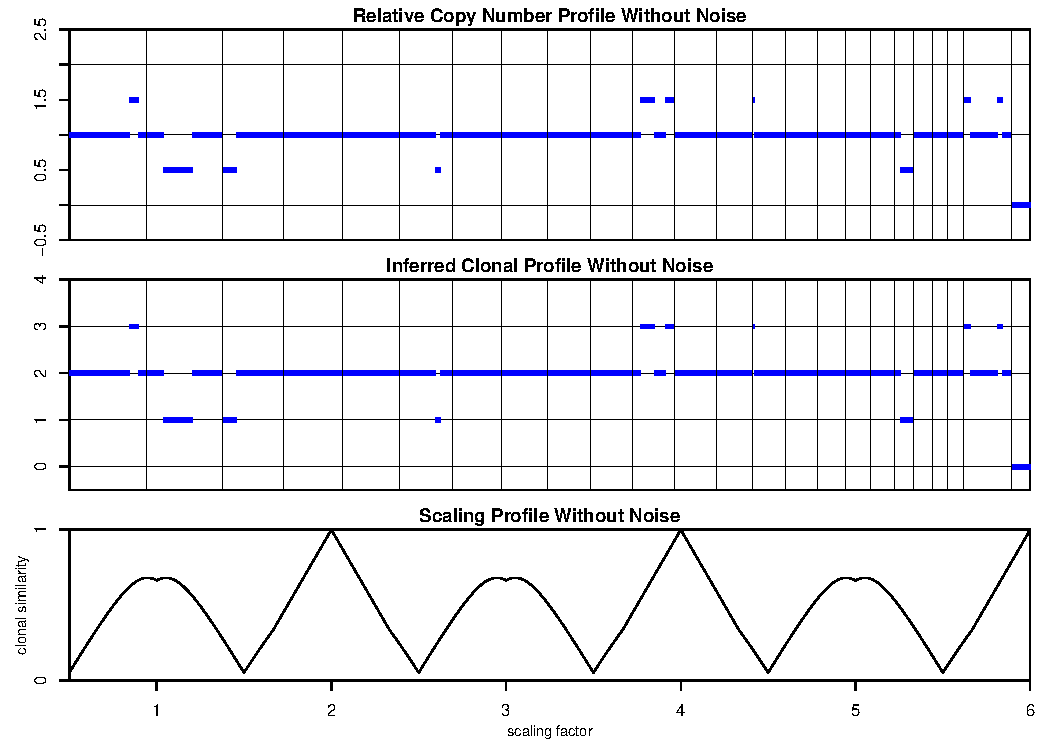
\includegraphics[width=.95\linewidth]{figure/unnamed-chunk-9-1} 
\begin{kframe}\begin{verbatim}
## scaling: 2 4 6 clonal similarity: 1
\end{verbatim}
\end{kframe}
\end{knitrout}
\caption{Relative (top) and inferred absolute (middle) copy number profiles for a simulation of 10 single copy number changes. Bottom: clonal similarity as a function of scaling. The inferred scaling factor is correctly 2, but with multiples of 2 giving equally good fits.}
\label{fig:rel_nonoise}
\end{figure}

The clonal similarity profile is in this case periodic with a period of 2, which is a consequence of the fact there there is no noise in the underlying data.

\newpage

\section*{8\quad Converting Noisy and Multiploid Relative Copy Numbers to Absolute}
We see that in the case with no noise, scaling factors of 2, 4, 6 etc. provide equally good clonal profiles. However, we can resolve this degeneracy in the case of noisy data. In this case we can write
\begin{equation*}
R = \alpha S + \beta
\end{equation*}
where R is our relative signal, S is the true signal and $\beta$ is noise. This implies
\begin{equation*}
S = \frac{R}{\alpha} - \frac{\beta}{\alpha}
\end{equation*}
Now setting $\frac{1}{\tilde{\alpha}} = 2\frac{1}{\alpha}$ we double the noise term leading to a worse fit to a clonal profile. This is exemplified in figure \ref{fig:rel_noise} which is similar to figure \ref{fig:rel_nonoise} except that it includes Gaussian noise and we no longer show the relative copy number profile. We see that in this case, scaling by 2 gives a uniquely good clonal similarity since a scaling of 4 increases the noise term.

\begin{figure}[h!]
  \centering
\begin{knitrout}
\definecolor{shadecolor}{rgb}{0.969, 0.969, 0.969}\color{fgcolor}\begin{kframe}
\begin{alltt}
\hlstd{res4} \hlkwb{=} \hlkwd{cnv_sim} \hlstd{(}\hlnum{10}\hlstd{,} \hlkwc{n_change} \hlstd{=} \hlnum{1}\hlstd{,} \hlkwc{noise} \hlstd{=} \hlnum{1}\hlstd{,} \hlkwc{ploidy}\hlstd{=}\hlnum{2}\hlstd{)}
\hlstd{res4_norm} \hlkwb{=} \hlkwd{normalize}\hlstd{(res4)}
\end{alltt}
\begin{verbatim}
## normalized data by 1.99
\end{verbatim}
\begin{alltt}
\hlstd{shift4} \hlkwb{=} \hlkwd{test_proximity}\hlstd{(res4_norm,} \hlkwc{main} \hlstd{=} \hlstr{'With Gaussian Noise'}\hlstd{)}
\end{alltt}
\end{kframe}
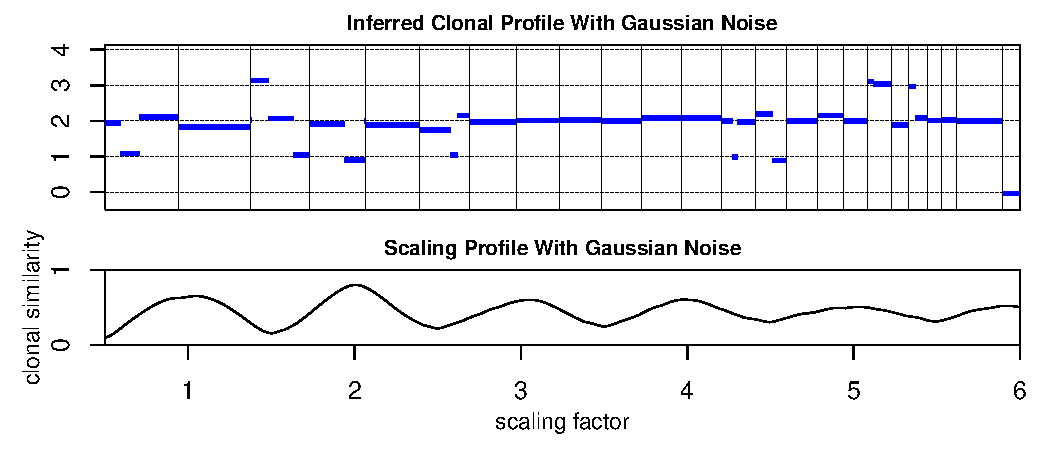
\includegraphics[width=.95\linewidth]{figure/unnamed-chunk-10-1} 
\begin{kframe}\begin{verbatim}
## scaling: 2.005 clonal similarity: 0.800448
\end{verbatim}
\end{kframe}
\end{knitrout}
\caption{Top: inferred absolute copy number profile for a simulation of 10 single copy number changes with Gaussian noise. Bottom: clonal similarity as a function of scaling. The inferred scaling factor is unique and correctly has a value of approximately 2.}
\label{fig:rel_noise}
\end{figure}

\newpage
Given the above considerations, we may also ask whether our proposed procedure can be used to infer correct absolute copy numbers when the reference genome is not diploid or when more copy number changes have occurred. In figure \ref{fig:triploid} we therefore perform a similar analysis generating 20 copy number changes from a triploid reference genome and in figure \ref{fig:rel_tetra} 50 copy number changes from a tetraploid reference genome allowing for changes of up to two copies per copy number change.

\begin{figure}[h!]
  \centering
\begin{knitrout}
\definecolor{shadecolor}{rgb}{0.969, 0.969, 0.969}\color{fgcolor}\begin{kframe}
\begin{alltt}
\hlstd{res5} \hlkwb{=} \hlkwd{cnv_sim} \hlstd{(}\hlnum{20}\hlstd{,} \hlkwc{n_change} \hlstd{=} \hlnum{1}\hlstd{,} \hlkwc{noise} \hlstd{=} \hlnum{1}\hlstd{,} \hlkwc{ploidy}\hlstd{=}\hlnum{3}\hlstd{)}
\hlstd{res5_norm} \hlkwb{=} \hlkwd{normalize}\hlstd{(res5)}
\end{alltt}
\begin{verbatim}
## normalized data by 3.06
\end{verbatim}
\begin{alltt}
\hlstd{shift5} \hlkwb{=} \hlkwd{test_proximity}\hlstd{(res5_norm,} \hlkwc{main} \hlstd{=} \hlstr{'Triploid'}\hlstd{)}
\end{alltt}
\end{kframe}
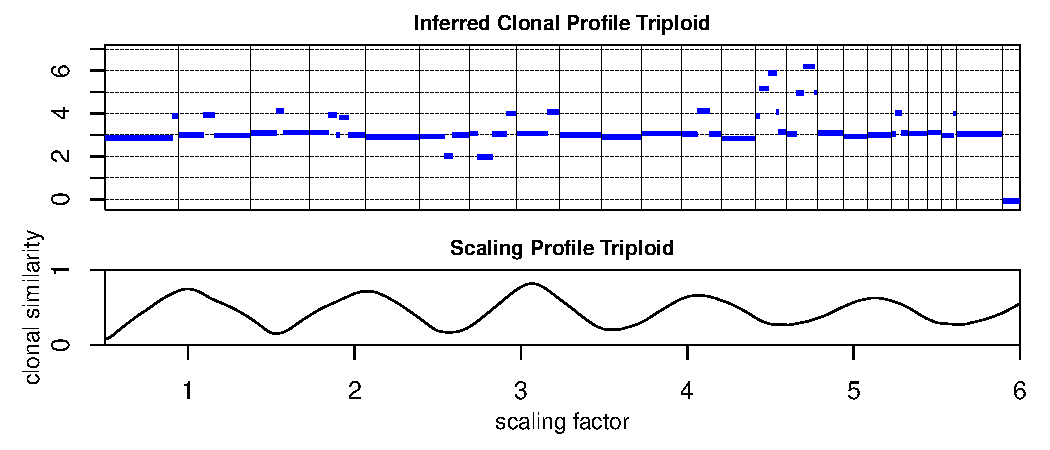
\includegraphics[width=.95\linewidth]{figure/unnamed-chunk-11-1} 
\begin{kframe}\begin{verbatim}
## scaling: 3.065 clonal similarity: 0.8195685
\end{verbatim}
\end{kframe}
\end{knitrout}
\caption{Top: inferred absolute copy number profile for a simulation of 20 single copy number changes with Gaussian noise and a triploid reference genome. Bottom: clonal similarity as a function of scaling. The inferred scaling factor is unique and correctly has a value of approximately 3, reflecting the triploid reference genome.}
\label{fig:triploid}
\end{figure}

\newpage

\begin{figure}[h!]
  \centering
\begin{knitrout}
\definecolor{shadecolor}{rgb}{0.969, 0.969, 0.969}\color{fgcolor}\begin{kframe}
\begin{alltt}
\hlstd{res6} \hlkwb{=} \hlkwd{cnv_sim} \hlstd{(}\hlnum{50}\hlstd{,} \hlkwc{n_change} \hlstd{=} \hlnum{2}\hlstd{,} \hlkwc{noise} \hlstd{=} \hlnum{1}\hlstd{,} \hlkwc{ploidy}\hlstd{=}\hlnum{4}\hlstd{)}
\hlstd{res6_norm} \hlkwb{=} \hlkwd{normalize}\hlstd{(res6)}
\end{alltt}
\begin{verbatim}
## normalized data by 3.91
\end{verbatim}
\begin{alltt}
\hlstd{shift6} \hlkwb{=} \hlkwd{test_proximity}\hlstd{(res6_norm,} \hlkwc{main} \hlstd{=} \hlstr{'Tetraploid'}\hlstd{)}
\end{alltt}
\end{kframe}
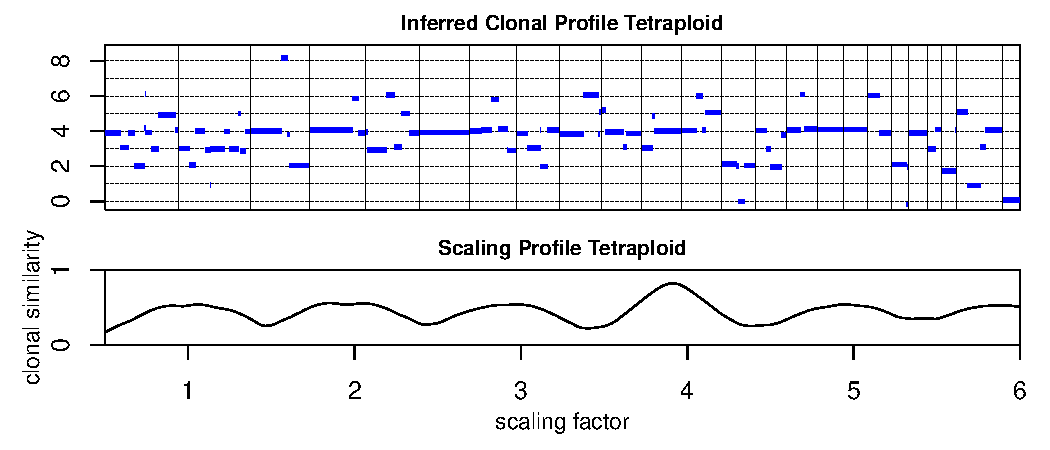
\includegraphics[width=.95\linewidth]{figure/unnamed-chunk-12-1} 
\begin{kframe}\begin{verbatim}
## scaling: 3.91 clonal similarity: 0.8231187
\end{verbatim}
\end{kframe}
\end{knitrout}
\caption{Top: Inferred absolute copy number profile for a simulation of 50 single copy number changes with Gaussian noise, a tetraploid reference genome, and allowing for copy number changes of up to two per event. Bottom: clonal similarity as a function of scaling. The inferred scaling factor is unique and correctly has a value of approximately 4, reflecting the tetraploid reference genome.}
\label{fig:rel_tetra}
\end{figure}

We see that in every case, we are able to correctly recover our absolute copy number profile from the relative copy number dataset, suggesting that this methodology is applicable to a range of different scenarios.

\newpage

\section*{9\quad Analysing Real Data}

Having seen that optimizing our proposed clonal similarity metric does indeed recover our original absolute copy numbers, we use a similar strategy to generate absolute copy number profiles for the experimental datasets provided.

As the data is given in the format [chromosome, start, end, cn], we first convert it to a dataframe of [chromosome, length, cn] for compatibility with previously described functions. This is achieved with the function parse\_segs(), which also fills in regions for which we do not have copy number information with NA. As this function is not part of the main report it is given in the appendix together with the function length\_to\_sec() which performs the opposite data conversion.



\begin{knitrout}
\definecolor{shadecolor}{rgb}{0.969, 0.969, 0.969}\color{fgcolor}\begin{kframe}
\begin{alltt}
\hlstd{segs} \hlkwb{=} \hlkwd{readRDS}\hlstd{(}\hlstr{'relative_segment_tables.rds'}\hlstd{)}
\hlstd{news} \hlkwb{=} \hlkwd{parse_segs}\hlstd{(segs)}
\end{alltt}
\end{kframe}
\end{knitrout}

For each of the five samples provided, we can now run the test\_proximity() function.

\begin{figure}[h!]
  \centering
\begin{knitrout}
\definecolor{shadecolor}{rgb}{0.969, 0.969, 0.969}\color{fgcolor}\begin{kframe}
\begin{alltt}
\hlstd{rds_1} \hlkwb{=} \hlkwd{test_proximity}\hlstd{(news[[}\hlnum{1}\hlstd{]],} \hlkwc{main} \hlstd{=} \hlkwd{names}\hlstd{(news)[}\hlnum{1}\hlstd{])}
\end{alltt}
\end{kframe}
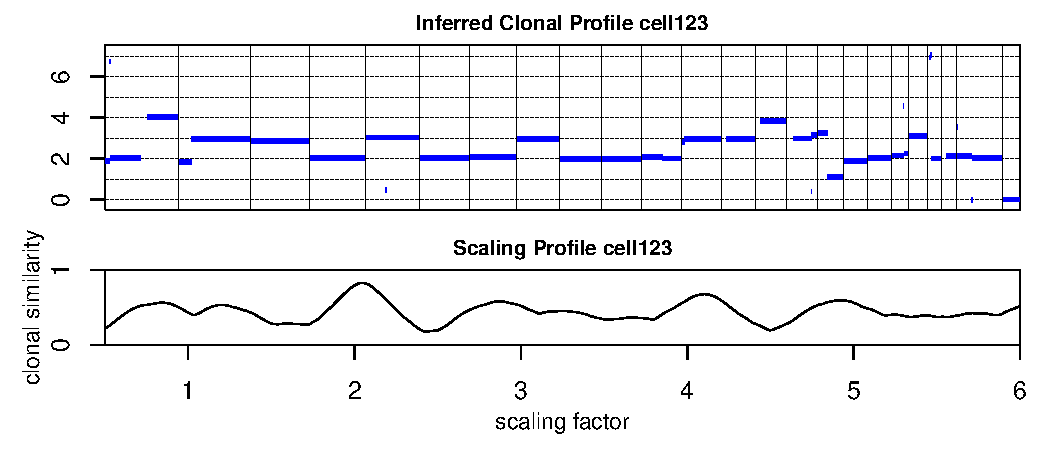
\includegraphics[width=.95\linewidth]{figure/unnamed-chunk-15-1} 
\begin{kframe}\begin{verbatim}
## scaling: 2.045 clonal similarity: 0.8288114
\end{verbatim}
\end{kframe}
\end{knitrout}
\caption{Inferred absolute copy number profile (top) and scaling profile (bottom) for experimental sample 1.}
\label{fig:samp1}
\end{figure}

We see that for cell123 using a scaling factor of very close to 2, we obtain a high clonal similarity of 0.83 and a genome that appears to be diploid but with significant genome duplications. These consist mostly of complete duplications of individual chromosomes.

\newpage


\begin{figure}[h!]
  \centering
\begin{knitrout}
\definecolor{shadecolor}{rgb}{0.969, 0.969, 0.969}\color{fgcolor}\begin{kframe}
\begin{alltt}
\hlstd{rds_2} \hlkwb{=} \hlkwd{test_proximity}\hlstd{(news[[}\hlnum{2}\hlstd{]],} \hlkwc{main} \hlstd{=} \hlkwd{names}\hlstd{(news)[}\hlnum{2}\hlstd{])}
\end{alltt}
\end{kframe}
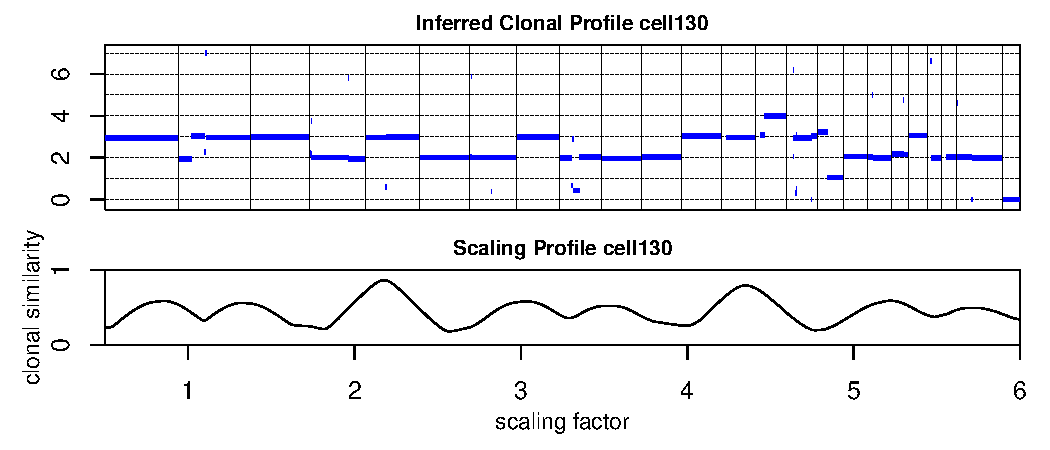
\includegraphics[width=.95\linewidth]{figure/unnamed-chunk-16-1} 
\begin{kframe}\begin{verbatim}
## scaling: 2.175 clonal similarity: 0.8633433
\end{verbatim}
\end{kframe}
\end{knitrout}
\caption{Inferred absolute copy number profile (top) and scaling profile (bottom) for experimental sample 2.}
\label{fig:samp2}
\end{figure}

cell130 has a clear peak at a scaling factor of 2.175, giving again a high clonal similarity of 0.86 and what appears to be either a diploid genome with significant genome duplications or a triploid genome with large deletions.

\begin{figure}[h!]
  \centering
\begin{knitrout}
\definecolor{shadecolor}{rgb}{0.969, 0.969, 0.969}\color{fgcolor}\begin{kframe}
\begin{alltt}
\hlstd{rds_3} \hlkwb{=} \hlkwd{test_proximity}\hlstd{(news[[}\hlnum{3}\hlstd{]],} \hlkwc{main} \hlstd{=} \hlkwd{names}\hlstd{(news)[}\hlnum{3}\hlstd{])}
\end{alltt}
\end{kframe}
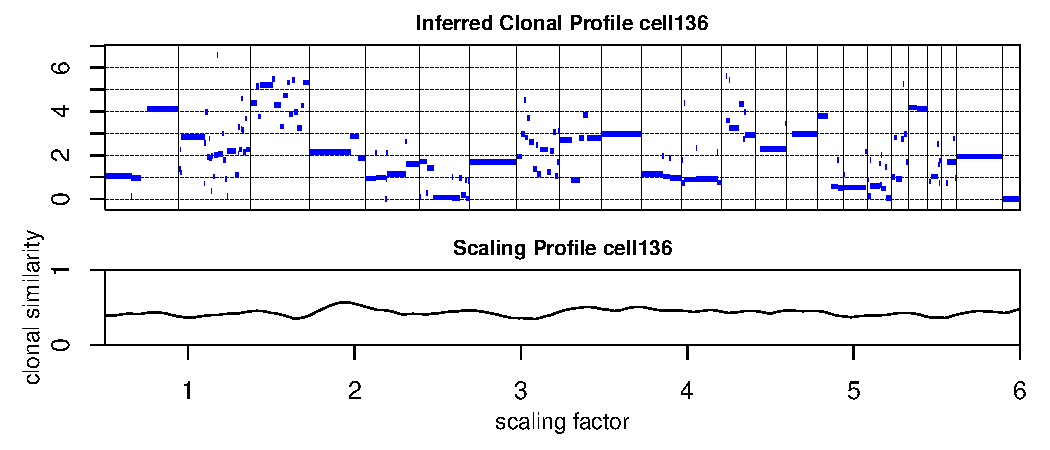
\includegraphics[width=.95\linewidth]{figure/unnamed-chunk-17-1} 
\begin{kframe}\begin{verbatim}
## scaling: 1.945 clonal similarity: 0.5684777
\end{verbatim}
\end{kframe}
\end{knitrout}
\caption{Inferred absolute copy number profile (top) and scaling profile (bottom) for experimental sample 3.}
\label{fig:samp3}
\end{figure}

cell136 does not have a very clear clonal similarity peak, and the optimum scaling factor of 1.945 only gives a clonal similarity of 0.568. We are thus not particularly confident in our estimated absolute copy number profile for this sample. Looking at the inferred copy number profile we observe that it is very fragmented with fragments at an almost continous range of copy numbers, explaining our difficulty in accurately assigning absolute copy numbers. However, we note that the major fragments seem to be separated in copy number by approximately integer values, lending support to our proposed scaling of approximately 2.

\begin{figure}[h!]
  \centering
\begin{knitrout}
\definecolor{shadecolor}{rgb}{0.969, 0.969, 0.969}\color{fgcolor}\begin{kframe}
\begin{alltt}
\hlstd{rds_4} \hlkwb{=} \hlkwd{test_proximity}\hlstd{(news[[}\hlnum{4}\hlstd{]],} \hlkwc{main} \hlstd{=} \hlkwd{names}\hlstd{(news)[}\hlnum{4}\hlstd{])}
\end{alltt}
\end{kframe}
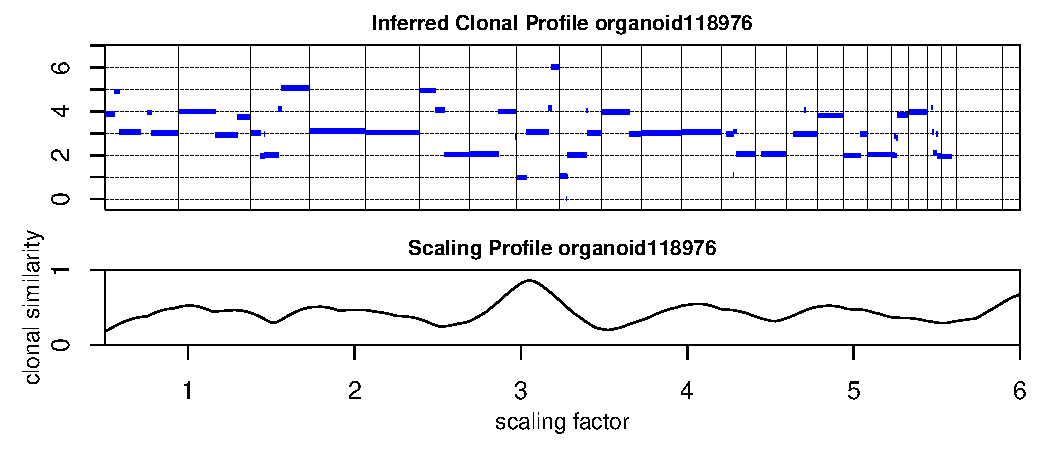
\includegraphics[width=.95\linewidth]{figure/unnamed-chunk-18-1} 
\begin{kframe}\begin{verbatim}
## scaling: 3.055 clonal similarity: 0.8590133
\end{verbatim}
\end{kframe}
\end{knitrout}
\caption{Inferred absolute copy number profile (top) and scaling profile (bottom) for experimental sample 4.}
\label{fig:samp4}
\end{figure}

For organoid118976 we observe larger copy number fragments and get a very clear peak at a scaling factor of 3.055 with a high clonal similarity of 0.86. This suggests that we could be looking at a triploid reference genome with various copy number gains and losses.

\newpage

\begin{figure}[h!]
  \centering
\begin{knitrout}
\definecolor{shadecolor}{rgb}{0.969, 0.969, 0.969}\color{fgcolor}\begin{kframe}
\begin{alltt}
\hlstd{rds_5} \hlkwb{=} \hlkwd{test_proximity}\hlstd{(news[[}\hlnum{5}\hlstd{]],} \hlkwc{main} \hlstd{=} \hlkwd{names}\hlstd{(news)[}\hlnum{5}\hlstd{])}
\end{alltt}
\end{kframe}
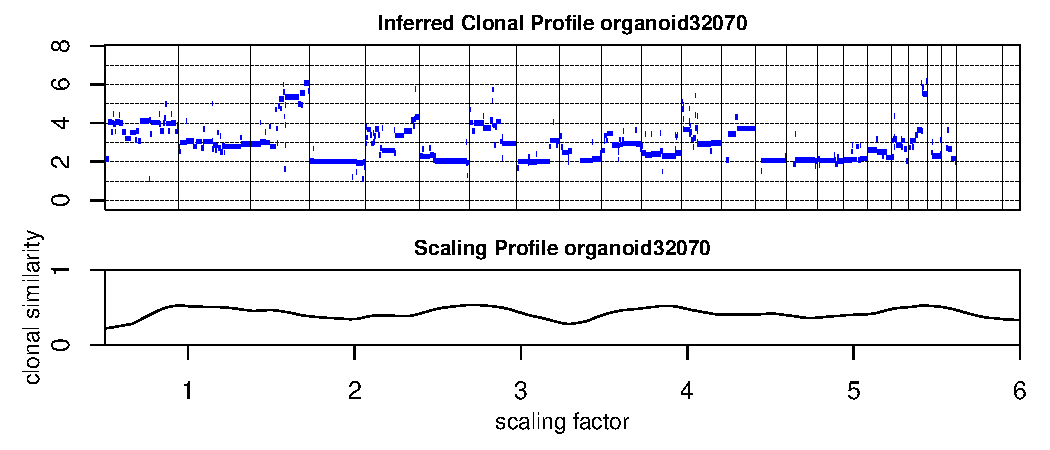
\includegraphics[width=.95\linewidth]{figure/unnamed-chunk-19-1} 
\begin{kframe}\begin{verbatim}
## scaling: 2.72 clonal similarity: 0.5343449
\end{verbatim}
\end{kframe}
\end{knitrout}
\caption{Inferred absolute copy number profile (top) and scaling profile (bottom) for experimental sample 5.}
\label{fig:samp5}
\end{figure}

For organoid32070 there is very little difference between scaling factors of 1.8, 2.7, and 3.8 which all give rise to relatively modest clonal similarities of approximately 0.53. We are thus again not particularly confident in our absolute copy number estimates.\\

To further investigate cell136 and organoid32070 where we do not appear to get a confident estimate of absolute copy numbers, we use a slightly different apporach where we also allow for an additive shift in the signal (figures \ref{fig:samp3_shift} \& \ref{fig:samp5_shift}). This corresponds to accounting for additive noise, based on the assumption that our experimental signal has the approximate form $R = \alpha S + \beta$. Assuming $\beta$ to include baseline noise, we expect to have to subtract noise from our relative signal to obtain the true signal and therefore let the shift parameter run from -0.3 to +0.05. This corresponds to allowing for $\beta$ values from -0.05 to 0.3. This is achieved with the function test\_proximity\_ss() which is exceedingly similar to test\_proximity() in its structure, and it is therefore included in the appendix rather than the main text.\\

\begin{figure}[h!]
  \centering
\begin{knitrout}
\definecolor{shadecolor}{rgb}{0.969, 0.969, 0.969}\color{fgcolor}\begin{kframe}
\begin{alltt}
\hlstd{rds_3} \hlkwb{=} \hlkwd{test_proximity_ss}\hlstd{(news[[}\hlnum{3}\hlstd{]],} \hlkwc{main} \hlstd{=} \hlkwd{names}\hlstd{(news)[}\hlnum{3}\hlstd{])}
\end{alltt}
\end{kframe}
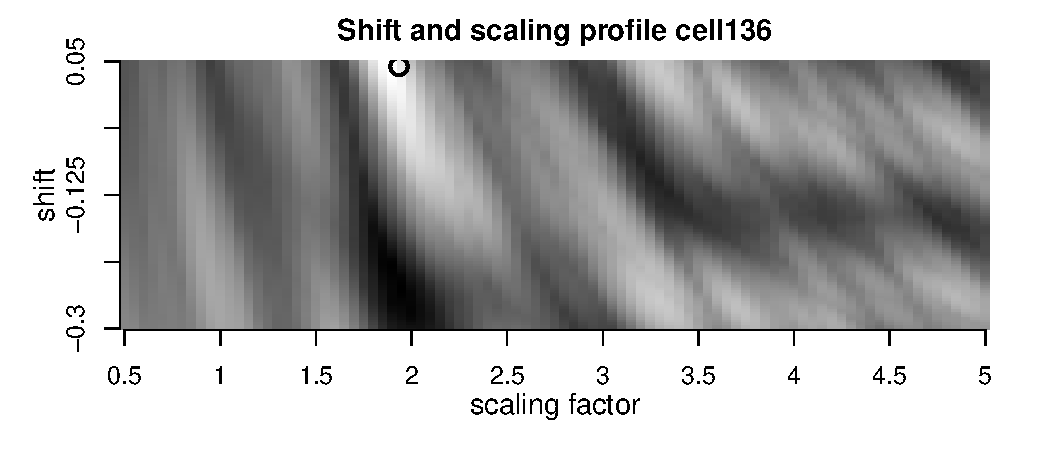
\includegraphics[width=.95\linewidth]{figure/unnamed-chunk-20-1} 
\begin{kframe}\begin{verbatim}
## shift: 0.043 scale: 1.9 clonal similarity: 0.5831508
\end{verbatim}
\end{kframe}
\end{knitrout}
\caption{Heatmap illustrating the dependence of clonal similarity on the shift and scaling used to generate an absolute copy number profile for experimental sample 3. Black circle indicates point of maximum clonal similarity.}
\label{fig:samp3_shift}
\end{figure}

\begin{figure}[h!]
  \centering
\begin{knitrout}
\definecolor{shadecolor}{rgb}{0.969, 0.969, 0.969}\color{fgcolor}\begin{kframe}
\begin{alltt}
\hlstd{rds_5} \hlkwb{=} \hlkwd{test_proximity_ss}\hlstd{(news[[}\hlnum{5}\hlstd{]],} \hlkwc{main} \hlstd{=} \hlkwd{names}\hlstd{(news)[}\hlnum{5}\hlstd{])}
\end{alltt}
\end{kframe}
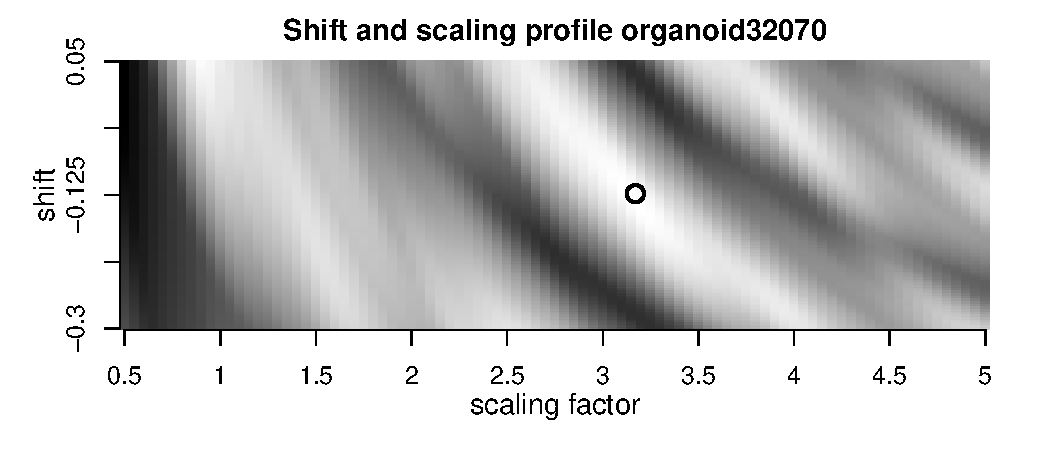
\includegraphics[width=.95\linewidth]{figure/unnamed-chunk-21-1} 
\begin{kframe}\begin{verbatim}
## shift: -0.125 scale: 3.15 clonal similarity: 0.5487136
\end{verbatim}
\end{kframe}
\end{knitrout}
\caption{Heatmap illustrating the dependence of clonal similarity on the shift and scaling used to generate an absolute copy number profile for experimental sample 5. Black circle indicates point of maximum clonal similarity.}
\label{fig:samp5_shift}
\end{figure}

We see that allowing for a shift in copy number prior to scaling does allow us to improve our clonal similarities, suggesting a better fit to a clonal profile. We also note that the scaling parameters change only modestly from to 1.945 to 1.9 for sample 3 and from 2.72 to 3.15 for sample 5. That is, the scalings remain near the same integer values with and without additive noise, and the two methods thus suggest similar ploidies for the reference genomes.\\

In summary we find that by optimizing a Euclidean clonal similarity metric, we can recover absolute copy number profiles from simulated relative copy number profiles. This is true for both diploid and multiploid reference genomes, a range of different copy number changes, and when including Gaussian noise. When applying this methodology to experimental data, we similarly recover clonal copy number profiles with a high clonal similarity for a number of samples. Two samples have low maximum clonal similarities with no clear peak, suggesting that the present method does not give a reliable absolute copy number profile for these samples. However, this can be partially remedied by allowing for a shift in the copy number data, accounting for e.g. a systematic baseline signal.

\newpage
\newpage
\newpage\newpage

\section*{Appendix}

\begin{knitrout}
\definecolor{shadecolor}{rgb}{0.969, 0.969, 0.969}\color{fgcolor}\begin{kframe}
\begin{alltt}
\hlstd{parse_segs} \hlkwb{=} \hlkwa{function}\hlstd{(}\hlkwc{segs}\hlstd{)\{}
  \hlcom{#given a list of dataframes with structure [chr, start, end, cn]}
  \hlcom{#returns a list of dataframes with structure [chr, length, cn]}
  \hlcom{#fills in segments for which we don't have data with NA}

  \hlstd{newsegs} \hlkwb{=} \hlkwd{list}\hlstd{()}
  \hlstd{chr_sizes} \hlkwb{=} \hlkwd{read.table}\hlstd{(chr_size_file)}
  \hlkwa{for} \hlstd{(i} \hlkwa{in} \hlnum{1}\hlopt{:}\hlkwd{length}\hlstd{(segs))\{}
    \hlstd{seg} \hlkwb{=} \hlstd{segs[[i]]}
    \hlstd{seg[,}\hlstr{'start'}\hlstd{]} \hlkwb{=} \hlkwd{as.numeric}\hlstd{(seg[,}\hlstr{'start'}\hlstd{])}
    \hlstd{seg[,}\hlstr{'end'}\hlstd{]} \hlkwb{=} \hlkwd{as.numeric}\hlstd{(seg[,}\hlstr{'end'}\hlstd{])}
    \hlstd{seg[,}\hlstr{'cn'}\hlstd{]} \hlkwb{=} \hlkwd{as.numeric}\hlstd{(seg[,}\hlstr{'cn'}\hlstd{])}

    \hlkwa{for} \hlstd{(j} \hlkwa{in} \hlkwd{c}\hlstd{(}\hlnum{1}\hlopt{:}\hlnum{22}\hlstd{,}\hlstr{'X'}\hlstd{,}\hlstr{'Y'}\hlstd{))\{} \hlcom{#standardize chromosome labels}
      \hlstd{seg[seg[,}\hlstr{'chr'}\hlstd{]} \hlopt{==} \hlstd{j,} \hlstr{'chr'}\hlstd{]} \hlkwb{=} \hlkwd{paste0}\hlstd{(}\hlstr{'chr'}\hlstd{,j)}
    \hlstd{\}}
    \hlstd{newseg} \hlkwb{=} \hlkwd{data.frame}\hlstd{(}\hlstr{'chr'} \hlstd{=} \hlkwd{c}\hlstd{(seg[}\hlnum{1}\hlstd{,}\hlstr{'chr'}\hlstd{]),}
                        \hlstr{'length'} \hlstd{=} \hlkwd{c}\hlstd{(seg[}\hlnum{1}\hlstd{,}\hlstr{'end'}\hlstd{]} \hlopt{-} \hlstd{seg[}\hlnum{1}\hlstd{,}\hlstr{'start'}\hlstd{]}\hlopt{+}\hlnum{1}\hlstd{),}
                        \hlstr{'cn'} \hlstd{=} \hlkwd{c}\hlstd{(seg[}\hlnum{1}\hlstd{,}\hlstr{'cn'}\hlstd{]),} \hlkwc{stringsAsFactors} \hlstd{=} \hlnum{FALSE}\hlstd{)}
    \hlkwa{if} \hlstd{(seg[}\hlnum{1}\hlstd{,}\hlstr{'start'}\hlstd{]} \hlopt{!=} \hlnum{1}\hlstd{)\{} \hlcom{#if we don't have data for beginning of chr1, add NA}
      \hlstd{newseg} \hlkwb{=} \hlkwd{rbind}\hlstd{(}\hlkwd{list}\hlstd{(seg[}\hlnum{1}\hlstd{,}\hlstr{'chr'}\hlstd{], seg[}\hlnum{1}\hlstd{,}\hlstr{'start'}\hlstd{]}\hlopt{-}\hlnum{1}\hlstd{,}  \hlnum{NA}\hlstd{), newseg)}
    \hlstd{\}}
    \hlkwa{if} \hlstd{((seg[}\hlnum{1}\hlstd{,}\hlstr{'end'}\hlstd{]}\hlopt{+}\hlnum{1} \hlopt{!=} \hlstd{seg[}\hlnum{2}\hlstd{,}\hlstr{'start'}\hlstd{])} \hlopt{&} \hlstd{(seg[}\hlnum{1}\hlstd{,} \hlstr{'chr'}\hlstd{]} \hlopt{==} \hlstd{seg[}\hlnum{2}\hlstd{,} \hlstr{'chr'}\hlstd{]))\{}
      \hlcom{#if we have a gap between segments, add NA}
      \hlstd{newseg} \hlkwb{=} \hlkwd{rbind}\hlstd{(newseg,} \hlkwd{list}\hlstd{(seg[}\hlnum{1}\hlstd{,}\hlstr{'chr'}\hlstd{],}
                                  \hlstd{seg[}\hlnum{2}\hlstd{,}\hlstr{'start'}\hlstd{]} \hlopt{-} \hlstd{seg[}\hlnum{1}\hlstd{,}\hlstr{'end'}\hlstd{]}\hlopt{-}\hlnum{1}\hlstd{,}  \hlnum{NA}\hlstd{))}
    \hlstd{\}}
    \hlkwa{for} \hlstd{(n} \hlkwa{in} \hlnum{2}\hlopt{:}\hlstd{(}\hlkwd{dim}\hlstd{(seg)[}\hlnum{1}\hlstd{]}\hlopt{-}\hlnum{1}\hlstd{))\{} \hlcom{#run through segments}
      \hlkwa{if} \hlstd{(seg[n,} \hlstr{'chr'}\hlstd{]} \hlopt{!=} \hlstd{seg[n}\hlopt{-}\hlnum{1}\hlstd{,} \hlstr{'chr'}\hlstd{])\{}
        \hlcom{#if new chromsome}
        \hlkwa{if} \hlstd{(seg[n,}\hlstr{'start'}\hlstd{]} \hlopt{!=} \hlnum{1}\hlstd{)\{} \hlcom{#if no data for beginning of chr, add NA}
          \hlstd{newseg} \hlkwb{=} \hlkwd{rbind}\hlstd{(newseg,} \hlkwd{list}\hlstd{(seg[n,}\hlstr{'chr'}\hlstd{], seg[n,}\hlstr{'start'}\hlstd{]}\hlopt{-}\hlnum{1}\hlstd{,}  \hlnum{NA}\hlstd{))}
        \hlstd{\}}
      \hlstd{\}}
      \hlstd{newseg} \hlkwb{=} \hlkwd{rbind}\hlstd{(newseg,}
                     \hlkwd{list}\hlstd{(seg[n,}\hlstr{'chr'}\hlstd{], seg[n,}\hlstr{'end'}\hlstd{]} \hlopt{-} \hlstd{seg[n,}\hlstr{'start'}\hlstd{]}\hlopt{+}\hlnum{1}\hlstd{,}
                     \hlstd{seg[n,}\hlstr{'cn'}\hlstd{]))}
      \hlkwa{if} \hlstd{((seg[n,}\hlstr{'end'}\hlstd{]}\hlopt{+}\hlnum{1} \hlopt{!=} \hlstd{seg[n}\hlopt{+}\hlnum{1}\hlstd{,}\hlstr{'start'}\hlstd{])} \hlopt{&}
          \hlstd{(seg[n,} \hlstr{'chr'}\hlstd{]} \hlopt{==} \hlstd{seg[n}\hlopt{+}\hlnum{1}\hlstd{,} \hlstr{'chr'}\hlstd{]))\{}
        \hlcom{#if we have a gap between segments, add NA}
        \hlstd{newseg} \hlkwb{=} \hlkwd{rbind}\hlstd{(newseg,} \hlkwd{list}\hlstd{(seg[n,}\hlstr{'chr'}\hlstd{],}
                        \hlstd{seg[n}\hlopt{+}\hlnum{1}\hlstd{,}\hlstr{'start'}\hlstd{]} \hlopt{-} \hlstd{seg[n,}\hlstr{'end'}\hlstd{]}\hlopt{-}\hlnum{1}\hlstd{,}  \hlnum{NA}\hlstd{))}
      \hlstd{\}}
      \hlkwa{if} \hlstd{(seg[n,} \hlstr{'chr'}\hlstd{]} \hlopt{!=} \hlstd{seg[n}\hlopt{+}\hlnum{1}\hlstd{,} \hlstr{'chr'}\hlstd{])\{}
        \hlcom{#if we don't have data for end of chr, add NA}
        \hlkwa{if} \hlstd{(seg[n,}\hlstr{'end'}\hlstd{]} \hlopt{!=} \hlstd{chr_sizes[chr_sizes[,}\hlnum{1}\hlstd{]} \hlopt{==} \hlstd{seg[n,}\hlstr{'chr'}\hlstd{],}\hlnum{2}\hlstd{])\{}
          \hlstd{newseg} \hlkwb{=} \hlkwd{rbind}\hlstd{(newseg,}\hlkwd{list}\hlstd{(seg[n,}\hlstr{'chr'}\hlstd{],}
                   \hlstd{chr_sizes[chr_sizes[,}\hlnum{1}\hlstd{]} \hlopt{==} \hlstd{seg[n,}\hlstr{'chr'}\hlstd{],}\hlnum{2}\hlstd{]}\hlopt{-}\hlstd{seg[n,}\hlstr{'end'}\hlstd{],}\hlnum{NA}\hlstd{))}
        \hlstd{\}}
      \hlstd{\}}
    \hlstd{\}}
    \hlcom{#fill out the rest of the final chromosome}
    \hlstd{newseg} \hlkwb{=} \hlkwd{rbind}\hlstd{(newseg,} \hlkwd{list}\hlstd{(seg[}\hlkwd{dim}\hlstd{(seg)[}\hlnum{1}\hlstd{],}\hlstr{'chr'}\hlstd{],}
                                \hlstd{seg[}\hlkwd{dim}\hlstd{(seg)[}\hlnum{1}\hlstd{],}\hlstr{'end'}\hlstd{]}\hlopt{-}\hlstd{seg[}\hlkwd{dim}\hlstd{(seg)[}\hlnum{1}\hlstd{],}\hlstr{'start'}\hlstd{]}\hlopt{+}\hlnum{1}\hlstd{,}
                                \hlstd{seg[}\hlkwd{dim}\hlstd{(seg)[}\hlnum{1}\hlstd{],}\hlstr{'cn'}\hlstd{]))}
    \hlkwa{if} \hlstd{(seg[}\hlkwd{dim}\hlstd{(seg)[}\hlnum{1}\hlstd{],}\hlstr{'end'}\hlstd{]} \hlopt{!=} \hlstd{chr_sizes[chr_sizes[,}\hlnum{1}\hlstd{]} \hlopt{==} \hlstd{seg[n,}\hlstr{'chr'}\hlstd{],}\hlnum{2}\hlstd{])\{}
      \hlstd{newseg} \hlkwb{=} \hlkwd{rbind}\hlstd{(newseg,} \hlkwd{list}\hlstd{(seg[}\hlkwd{dim}\hlstd{(seg)[}\hlnum{1}\hlstd{],}\hlstr{'chr'}\hlstd{],}
                                \hlstd{chr_sizes[chr_sizes[,}\hlnum{1}\hlstd{]}\hlopt{==}\hlstd{seg[}\hlkwd{dim}\hlstd{(seg)[}\hlnum{1}\hlstd{],}\hlstr{'chr'}\hlstd{],}\hlnum{2}\hlstd{]}
                                \hlopt{-}\hlstd{seg[}\hlkwd{dim}\hlstd{(seg)[}\hlnum{1}\hlstd{],}\hlstr{'end'}\hlstd{],} \hlnum{NA}\hlstd{))}
    \hlstd{\}}
    \hlstd{newsegs[[i]]} \hlkwb{=} \hlstd{newseg} \hlcom{#add to list of segments with new format}
  \hlstd{\}}
  \hlkwd{names}\hlstd{(newsegs)} \hlkwb{=} \hlkwd{names}\hlstd{(segs)}
  \hlkwd{return}\hlstd{(newsegs)}
\hlstd{\}}

\hlstd{length_to_seg} \hlkwb{=} \hlkwa{function}\hlstd{(}\hlkwc{results}\hlstd{)\{}
  \hlcom{#given a dataframe with structure [chr, length, cn]}
  \hlcom{#returns a dataframe with structure [chr, start, end, cn]}
  \hlstd{segs} \hlkwb{=} \hlkwd{data.frame}\hlstd{(}\hlstr{'chr'} \hlstd{=} \hlkwd{c}\hlstd{(results[}\hlnum{1}\hlstd{,}\hlstr{'chr'}\hlstd{]),} \hlstr{'start'} \hlstd{=} \hlkwd{c}\hlstd{(}\hlnum{1}\hlstd{),}
                    \hlstr{'end'} \hlstd{=} \hlkwd{c}\hlstd{(results[}\hlnum{1}\hlstd{,}\hlstr{'length'}\hlstd{]),} \hlstr{'cn'} \hlstd{=} \hlkwd{c}\hlstd{(results[}\hlnum{1}\hlstd{,}\hlstr{'cn'}\hlstd{]),}
                    \hlkwc{stringsAsFactors} \hlstd{=} \hlnum{0}\hlstd{)}
  \hlstd{x} \hlkwb{=} \hlstd{results[}\hlnum{1}\hlstd{,}\hlstr{'length'}\hlstd{]} \hlcom{#use x as positional counter along chromsome}

  \hlkwa{for} \hlstd{(i} \hlkwa{in} \hlnum{2}\hlopt{:}\hlkwd{dim}\hlstd{(results)[}\hlnum{1}\hlstd{])\{}
    \hlkwa{if} \hlstd{(results[i,} \hlstr{'chr'}\hlstd{]} \hlopt{==} \hlstd{results[i}\hlopt{-}\hlnum{1}\hlstd{,} \hlstr{'chr'}\hlstd{])\{} \hlcom{#if same chromosome}
      \hlstd{segs[i,]} \hlkwb{=} \hlkwd{list}\hlstd{(results[i,}\hlstr{'chr'}\hlstd{],x}\hlopt{+}\hlnum{1}\hlstd{,x}\hlopt{+}\hlstd{results[i,}\hlstr{'length'}\hlstd{],results[i,}\hlstr{'cn'}\hlstd{])}
      \hlstd{x} \hlkwb{=} \hlstd{x} \hlopt{+} \hlstd{results[i,} \hlstr{'length'}\hlstd{]}
    \hlstd{\}}\hlkwa{else}\hlstd{\{} \hlcom{#if starting new chromsome, reset counter}
      \hlstd{segs[i,]} \hlkwb{=} \hlkwd{list}\hlstd{(results[i,}\hlstr{'chr'}\hlstd{],} \hlnum{1}\hlstd{, results[i,}\hlstr{'length'}\hlstd{], results[i,}\hlstr{'cn'}\hlstd{])}
      \hlstd{x} \hlkwb{=} \hlstd{results[i,} \hlstr{'length'}\hlstd{]}
    \hlstd{\}}
  \hlstd{\}}
  \hlkwd{return}\hlstd{(segs)}
\hlstd{\}}

\hlstd{test_proximity_ss} \hlkwb{=} \hlkwa{function}\hlstd{(} \hlkwc{results}\hlstd{,} \hlkwc{scale_factors} \hlstd{=} \hlstr{'default'}\hlstd{,}
                              \hlkwc{shift_factors} \hlstd{=} \hlstr{'default'}\hlstd{,} \hlkwc{main}\hlstd{=}\hlstr{'default'} \hlstd{)\{}
  \hlcom{#finds absolute copy numbers using both scaling and shifting}
  \hlstd{res} \hlkwb{=} \hlstd{results[} \hlopt{!}\hlkwd{is.na}\hlstd{(results[,}\hlstr{'cn'}\hlstd{]), ]} \hlcom{#consider only segments with data}
  \hlkwa{if} \hlstd{(scale_factors} \hlopt{==} \hlstr{'default'}\hlstd{)\{}
    \hlstd{scale_factors} \hlkwb{=} \hlkwd{seq}\hlstd{(} \hlnum{0.5}\hlstd{,} \hlnum{5}\hlstd{,} \hlkwc{l}\hlstd{=}\hlnum{91} \hlstd{)} \hlcom{#go from .5ploid to pentaploid reference}
  \hlstd{\}}
  \hlkwa{if} \hlstd{(shift_factors} \hlopt{==} \hlstr{'default'}\hlstd{)\{}
    \hlstd{shift_factors} \hlkwb{=} \hlkwd{seq}\hlstd{(} \hlopt{-}\hlnum{0.3}\hlstd{,}\hlnum{0.05}\hlstd{,} \hlkwc{l}\hlstd{=}\hlnum{101}\hlstd{)} \hlcom{#assume noise is additive}
  \hlstd{\}}
  \hlstd{sims} \hlkwb{=} \hlkwd{matrix}\hlstd{(,}\hlkwd{length}\hlstd{(shift_factors),} \hlkwd{length}\hlstd{(scale_factors))}
  \hlstd{test_res}\hlkwb{=}\hlstd{res}
  \hlkwa{for} \hlstd{(shift} \hlkwa{in} \hlnum{1}\hlopt{:}\hlkwd{length}\hlstd{(shift_factors))\{}
    \hlkwa{for} \hlstd{(scale} \hlkwa{in} \hlnum{1}\hlopt{:}\hlkwd{length}\hlstd{(scale_factors))\{}
      \hlcom{#consider combinations of scalings and shifts}
      \hlstd{test_res[,}\hlstr{'cn'}\hlstd{]} \hlkwb{=} \hlstd{(res[,}\hlstr{'cn'}\hlstd{]}\hlopt{+}\hlstd{shift_factors[shift])}\hlopt{*}\hlstd{scale_factors[scale]}
      \hlstd{sim} \hlkwb{=} \hlkwd{clonal_proximity}\hlstd{(test_res)} \hlcom{#quantify clonal similarity}
      \hlstd{sims[shift,scale]} \hlkwb{=} \hlstd{sim} \hlcom{#store in matrix}
    \hlstd{\}}
  \hlstd{\}}

  \hlstd{simmax} \hlkwb{=} \hlkwd{max}\hlstd{(sims)}
  \hlstd{param_max} \hlkwb{=} \hlkwd{which}\hlstd{(sims}\hlopt{==}\hlstd{simmax,} \hlkwc{arr.ind}\hlstd{=}\hlnum{1}\hlstd{)} \hlcom{#find optimum shift & scaling}
  \hlstd{shiftmax} \hlkwb{=} \hlstd{shift_factors[param_max[}\hlnum{1}\hlstd{,}\hlnum{1}\hlstd{]]}
  \hlstd{scalemax} \hlkwb{=} \hlstd{scale_factors[param_max[}\hlnum{1}\hlstd{,}\hlnum{2}\hlstd{]]}

  \hlkwd{par}\hlstd{(} \hlkwc{mfrow} \hlstd{=} \hlkwd{c}\hlstd{(}\hlnum{1}\hlstd{,}\hlnum{1}\hlstd{),} \hlkwc{mar} \hlstd{=} \hlkwd{c}\hlstd{(}\hlnum{4}\hlstd{,}\hlnum{4}\hlstd{,}\hlnum{2}\hlstd{,}\hlnum{2}\hlstd{))}
  \hlcom{#plot heatmap of clonal similarities}
  \hlkwd{image}\hlstd{(}\hlkwd{t}\hlstd{(sims),} \hlkwc{xlab}\hlstd{=}\hlstr{''}\hlstd{,} \hlkwc{ylab}\hlstd{=}\hlstr{''}\hlstd{,} \hlkwc{axes}\hlstd{=}\hlnum{0}\hlstd{,} \hlkwc{col}\hlstd{=}\hlkwd{grey}\hlstd{(}\hlkwd{seq}\hlstd{(}\hlnum{0}\hlstd{,} \hlnum{1}\hlstd{,} \hlkwc{length} \hlstd{=} \hlnum{256}\hlstd{)),}
        \hlkwc{main} \hlstd{=} \hlkwd{paste0}\hlstd{(}\hlstr{'Shift and scaling profile '}\hlstd{, main) )}
  \hlkwd{axis}\hlstd{(}\hlnum{1}\hlstd{,} \hlkwc{at} \hlstd{=} \hlkwd{seq}\hlstd{(}\hlnum{0}\hlstd{,} \hlnum{1}\hlstd{,} \hlkwc{length} \hlstd{=} \hlnum{10}\hlstd{),}
       \hlkwc{labels}\hlstd{=}\hlkwd{seq}\hlstd{(scale_factors[}\hlnum{1}\hlstd{], scale_factors[}\hlkwd{length}\hlstd{(scale_factors)],} \hlkwc{l}\hlstd{=}\hlnum{10}\hlstd{)}
       \hlstd{,}\hlkwc{srt}\hlstd{=}\hlnum{45}\hlstd{,}\hlkwc{tick}\hlstd{=}\hlnum{TRUE}\hlstd{)}
  \hlkwd{axis}\hlstd{(}\hlnum{2}\hlstd{,} \hlkwc{at} \hlstd{=} \hlkwd{seq}\hlstd{(}\hlnum{0}\hlstd{,} \hlnum{1}\hlstd{,} \hlkwc{length} \hlstd{=} \hlnum{5}\hlstd{),}
       \hlkwc{labels}\hlstd{=}\hlkwd{seq}\hlstd{( shift_factors[}\hlnum{1}\hlstd{],shift_factors[}\hlkwd{length}\hlstd{(shift_factors)],} \hlkwc{l}\hlstd{=}\hlnum{5}\hlstd{)}
       \hlstd{,}\hlkwc{srt}\hlstd{=}\hlnum{45}\hlstd{,}\hlkwc{tick}\hlstd{=}\hlnum{TRUE}\hlstd{)}
  \hlkwd{title}\hlstd{(}\hlkwc{ylab}\hlstd{=}\hlstr{"shift"}\hlstd{,} \hlkwc{line}\hlstd{=}\hlnum{2}\hlstd{,} \hlkwc{cex.lab}\hlstd{=}\hlnum{1.2}\hlstd{)}
  \hlkwd{title}\hlstd{(}\hlkwc{xlab}\hlstd{=}\hlstr{"scaling factor"}\hlstd{,} \hlkwc{line}\hlstd{=}\hlnum{2}\hlstd{,} \hlkwc{cex.lab}\hlstd{=}\hlnum{1.2}\hlstd{)}
  \hlkwd{draw.circle}\hlstd{(param_max[}\hlnum{1}\hlstd{,}\hlnum{2}\hlstd{]}\hlopt{/}\hlkwd{length}\hlstd{(scale_factors),}
              \hlstd{param_max[}\hlnum{1}\hlstd{,}\hlnum{1}\hlstd{]}\hlopt{/}\hlkwd{length}\hlstd{(shift_factors),}
              \hlnum{0.01}\hlstd{,} \hlkwc{border}\hlstd{=}\hlstr{'black'}\hlstd{,} \hlkwc{lwd}\hlstd{=}\hlnum{2}\hlstd{)}

  \hlcom{#write a summary}
  \hlkwd{cat}\hlstd{(}\hlstr{'shift:'}\hlstd{, shiftmax,} \hlstr{'scale:'}\hlstd{, scalemax,}\hlstr{'clonal similarity:'}\hlstd{, simmax)}

  \hlkwd{return}\hlstd{(}\hlkwd{list}\hlstd{(}\hlstr{'results'}\hlstd{=results,} \hlstr{'scaling'}\hlstd{=scalemax,}
              \hlstr{'shift'}\hlstd{=shiftmax,} \hlstr{'clonal'}\hlstd{=simmax))}
\hlstd{\}}
\end{alltt}
\end{kframe}
\end{knitrout}


\end{document}
